%%%%%%%%%%%%%%%%%%%%%%%%%%%%%%%%%%%%%%%%%%%%%%%%%%%%%%%%%%%%%%%%%%% 
%                                                                 %
%                            ROOT FILE                            %
%                                                                 %
%%%%%%%%%%%%%%%%%%%%%%%%%%%%%%%%%%%%%%%%%%%%%%%%%%%%%%%%%%%%%%%%%%% 
%
%  Run LaTeX or pdfLaTeX on this file to produce your thesis.
%  To produce the abstract title page followed by the abstract,
%  see the file abstitle-phd.tex or abstitle-mas.tex.
%
%%%%%%%%%%%%%%%%%%%%%%%%%%%%%%%%%%%%%%%%%%%%%%%%%%%%%%%%%%%%%%%%%%%

\documentclass[chap,openright]{thesis}  %twoside,   12pt, 
% Use the first command below if you want captions over 1 line indented. A side
% effect of this is to remove the use of bold for captions (thesis default).
% To restore bold, also include the second line below.
%\usepackage[hang]{caption}      % to indent subsequent lines of captions
%\renewcommand{\captionfont}{\bfseries} % bold caption (needed with caption 
                                       % package to restore boldface.)
% \setstretch{1.5} 
% \renewcommand\chaptersize{\large}
% \renewcommand\sectionsize{\large}
% \renewcommand\subsectionsize{\normalsize}
% \renewcommand\subsubsectionsize{\normalsize}
% \renewcommand{\bibalign}{}

% \usepackage{subcaption}
%\captionsetup{compatibility=false}
% \usepackage{float}
% \usepackage{caption}
\bibliographystyle{IEEEtran_rpi}
\usepackage{amsmath}
\usepackage{amsfonts}
\usepackage{amssymb}
\usepackage{amsthm}
\usepackage{mathtools}
\usepackage{commath}
\usepackage{rotating}
\usepackage[linesnumbered,ruled]{algorithm2e}
\SetKwInOut{Parameter}{parameter}
\usepackage[textsize=small,textwidth=1.75in]{todonotes}
% \usepackage{setspace}
\usepackage{xspace} % needed for \eg, \ie, \etc
% hyperref must be last
%When submitting your thesis, comment out hyperref
% -- courtesy of Dan Ibanez
\usepackage[hidelinks]{hyperref}

\renewcommand*{\UrlNoBreaks}{\do\(\do\[\do\{\do\<\do\:}%

%\usepackage{hyperref}
%\hypersetup{
%  colorlinks=true,
%  linkcolor=blue,
%  citecolor=blue,
%  urlcolor=blue
%}
\usepackage{multirow}
\newtheorem{definition}{Definition}[section]
\newtheorem{theorem}{Theorem}
\newtheorem{remark}{Remark}

\usepackage{cleveref}
\usepackage{booktabs}
\usepackage{siunitx}
\usepackage{longtable}
\usepackage{array}
\usepackage{lscape}


\usepackage{graphicx}
\usepackage{float}
%\usepackage{subcaption}    % clashes with \subfig package below
\usepackage[caption=false]{subfig}
\usepackage{url}

\newcommand{\etal}[0]{{\em et~al.\@}\xspace}
\newcommand{\eg}[0]{{e.g.\@}\xspace}
\newcommand{\ie}[0]{{i.e.\@}\xspace}
\newcommand{\viz}[0]{{viz.\@}\xspace}
\newcommand{\resp}[0]{{resp.\@}\xspace}
\DeclareMathOperator{\mydiag}{diag}
\newcommand{\comment}[1]{}
\newcommand{\mat}[1]{\ensuremath{\mathsf{#1}}}
\newcommand{\nsig}[0]{\ensuremath{n_{\mat{\Sigma}}}}


\usepackage{lipsum}

\newcommand\blfootnote[1]{%
  \begingroup
  \renewcommand\thefootnote{}\footnote{#1}%
  \addtocounter{footnote}{-1}%
  \endgroup
}


% \PassOptionsToPackage{usenames,dvipsnames}{xcolor}

% \usepackage{colortbl}
% \newcommand{\padd}[1]{{\leavevmode\color{blue}{#1}}}

% \usepackage{color, colortbl}
%\definecolor{blue}{rgb}{0,0.75,1}
%\definecolor{yellow}{rgb}{1,1,0}

% \includeonly{rpichap1}  % use \includeonly to process only
                         % the file(s) listed inside the braces        
% \begin{singlespace}
% \end{singlespace}

     
\begin{document}
%%%%%%%%%%%%%%%%%%%%%%%%%%%%%%%%%%%%%%%%%%%%%%%%%%%%%%%%%%%%%%%%%%% 
%                                                                 %
%                            TITLE PAGE                           %
%                            PhD Thesis                           %
%                                                                 %
%%%%%%%%%%%%%%%%%%%%%%%%%%%%%%%%%%%%%%%%%%%%%%%%%%%%%%%%%%%%%%%%%%% 
%  This file produces the title page, copyright page (if requested)
%  and the Table of Contents, List of Figures and List of Tables.
% 
%  To produce the abstract title page followed by the abstract,
%  see the template file, "abstitle-phd.tex"
%%%%%%%%%%%%%%%%%%%%%%%%%%%%%%%%%%%%%%%%%%%%%%%%%%%%%%%%%%%%%%%%%%%
    
% Supply information for use on title page:
%   
\thesistitle{\bf A Matrix-free Algorithm \\for reduced-space PDE-constrained Optimization}        
\author{Pengfei Meng}        
\degree{Doctor of Philosophy}        
\department{Aeronautical Engineering} % provide your area of study here; e.g.,
%  "Mechanical Engineering", "Nuclear Engineering", "Physics", etc.   
     
\signaturelines{4}     %max number of signature lines is 7        
\thadviser{Jason E. Hicken}
 %\cothadviser{Second Adviser} % If you have 2 thesis advisers
\memberone{Assad A. Oberai}        
\membertwo{Lucy T. Zhang}        
\memberthree{John E. Mitchell}
%\memberfour{Marcus Aurelius} % must change signaturelines to 5 if using this 5 members
%\memberfive{Marcus Junius Brutus} % must change signaturelines to 6 if using this 6 members
%\membersix{Nikola Tesla} % must change signaturelines to 7 if using this 7 members

\submitdate{April 2018\\(For Graduation May 2018)}
\copyrightyear{2018}   % if omitted, current year is used.        

% Print titlepage and other prefatory material:
%    
\titlepage    
%\vfil
%\begin{flushleft}
%PhD life is nonlinear, most of the time it stays flat and boring, until it's not. 
%\end{flushleft}
%{\raggedleft Pengfei Meng \quad \par} 
%\vfil
\copyrightpage         % optional           
\tableofcontents        
\listoftables          % required if there are tables
\listoffigures         % required if there are figures


   
%%%%%%%%%%%%%%%%%%%%%%%%%%%%%%%%%%%%%%%%%%%%%%%%%%%%%%%%%%%%%%%%%%% 
%                                                                 %
%                         ACKNOWLEDGEMENT                         %
%                                                                 %
%%%%%%%%%%%%%%%%%%%%%%%%%%%%%%%%%%%%%%%%%%%%%%%%%%%%%%%%%%%%%%%%%%% 
 
\specialhead{ACKNOWLEDGMENT}
 
%This dissertation is the essence of the not-so-short four and half years' work in the Optimal Design Lab of Professor Jason E. Hicken at Rensselaer Polytechnic Institute.  The PhD experience has taught me numerous valuable lessons in doing research,  given me sharper insights in numerical optimization field, and confidence in doing whatever is waiting ahead.  

I would like to thank my advisor, Professor Jason E. Hicken, for the numerous discussions he patiently had with me 
for the past five years. His broad knowledge and insights in numerical simulation and design field continue to motivate me.  Beyond being professional, he is a very nice person to work with, and it is my pleasure to have him as my advisor. 

I thank my doctoral committee members, Prof. Assad A. Oberai, Prof. Lucy T. Zhang, Prof. John E. Mitchell for the time they spent on my candidacy and thesis defense. Their valuable inputs greatly help improve the quality of my thesis work. 

Many thanks to my fellow lab mates in CII lab for providing a lively and humorous environment: Alp Dener, Anthony Ashley,  Jared Crean, Jianfeng Yan, Kinshuk Panda. In particular, thank you to Alp Dener, whose work in Kona laid the foundation for my thesis research, and who very generously gave me numerous valuable suggestions. 

I gratefully acknowledge Dr. Gaetan Kenway, Dr. Charles (Sandy) Mader in MDO design lab at University of Michigan for their help with the CFD solver ADflow. 

Lastly I am grateful to have my family with me, Yongjian, and most recently Emma, my mom and my sister. 

%I am indebted to my mom for her constant support and love, despite the long distance and long time separation caused by my studying in the U.S.. My only sister, for the special bond we had through the rough days, and for your love and trust in me all the time. 
%
%Yongjian Yang, thank you for being my life companion, and the meanings and purposes you instill to my life. I am grateful for having my baby daughter Emma. Everyday is a surprise with you. The lively energy you emits is my greatest source of happiness and inspiration.  

This thesis is jointly funded by the NASA Learn project, Prof. Hicken's startup grant, and TA funding from the MANE department. Specially, thanks to OGE at RPI for supporting me with Childbirth Accommodation in fall 2017 after my baby was born, which enable me to spend more time with my baby and smoothly finish my PhD. 
   
%%%%%%%%%%%%%%%%%%%%%%%%%%%%%%%%%%%%%%%%%%%%%%%%%%%%%%%%%%%%%%%%%%% 
%                                                                 %
%                            ABSTRACT                             %
%                                                                 %
%%%%%%%%%%%%%%%%%%%%%%%%%%%%%%%%%%%%%%%%%%%%%%%%%%%%%%%%%%%%%%%%%%% 
 
\specialhead{ABSTRACT}
 In this thesis, a Reduced-Space Newton-Krylov method with Homotopy globalization technique is presented to solve PDE-constrained optimization problems.  
 
In the context of PDE-constrained optimization problems, besides the design variables, the state variables also come into play. The objective and some of the constraint functions would depend on both the design and state variables. The  
total derivatives of the state-based objective and constraints necessitate an adjoint solve for each, which can be as expensive as the PDE solves. In presence of many state-based constraints, it may not be practical to compute the constraint Jacobian explicitly. Besides, the dimension of PDE-constrained problems are usually very large, storing the Jacobian matrices put a heavy load on the computer memory.  A matrix-free Newton-Krylov optimization algorithm avoids these problems, but presents additional challenges related to globalization, preconditioning, and inequality constraint handling abilities. 

To address the former challenges, this thesis uses a globally convergent homotopy continuation approach to solve the first-order optimality conditions. It uses a predictor-corrector algorithm to trace the solution curve of the homotopy map that gathers the KKT condition and a homotopy regularization term. During the tracing process, the predictor and corrector linear systems are solved loosely by Krylov iterative methods. The necessary matrix-vector products of the KKT matrix are approximated using second-order adjoints. This way, the computational cost of calculating the constraint Jacobians and memory cost of storing them are saved.  To cope with the poorly conditioned KKT system, matrix-free preconditioners based on Lanczos SVD approximation are proposed to accelerate the convergence of the Krylov iterative solvers.  

The proposed algorithm and preconditions are tested on a variety of problems. To verify its non-convexity handling ability, a constructed quadratic indefinite problem is exercised. The scaling performance of the algorithm and the preconditioners is studied on a series of constructed quadratic problems with increasing dimensions, while the convergence results are compared with a popular matrix-based active-set optimization algorithm. The algorithm and preconditioners are also applied on a subset of CUTEr test problems to examine its accuracy and robustness. Finally, two PDE-constrained optimization problems are tested, the first one is a complex stress-constrained mass-minimization problem, which serves as the case with many state-based constraints, the second one is an aerodynamic shape of the NASA Common Research Model wing based on Euler equations. In both cases, the results using the algorithm and preconditioners from this work are compared with that using state-of-the-art matrix-based optimization algorithm SNOPT. 

%%%%%%%%%%%%%%%%%%%%%%% 
  
%%%%%%%%%%%%%%%%%%%%%%%%%%%%%%%%%%%%%%%%%%%%%%%%%%%%%%%%%%%%%%%%%%% 
%                                                                 %
%                            CHAPTER ONE                          %
%                                                                 %
%1.1: Big-picture motivation for design optimization
%1.2: What is PDE-constrained opt and why is it valuable for design?
%1.3: Why are conventional optimization algorithms not well suited for (reduced-space) PDE-constrained opt?
%1.4: Matrix-free NK methods: what are they and what are their advantages over conventional opt
%1.5: What are the challenges with using Matrix-free NK that need to be addressed?
%1.6: Thesis Contributions that relate to the challenges above.
%1.7: Thesis Outline
%%%%%%%%%%%%%%%%%%%%%%%%%%%%%%%%%%%%%%%%%%%%%%%%%%%%%%%%%%%%%%%%%%% 
 
\chapter{INTRODUCTION}\label{chap:1}
 
\section{Motivation}
Global warming has been unequivocally proven by scientific evidence~\cite{nasa_warm}. 
Furthermore, there is also strong evidence that human activities, especially anthropogentic emissions of carbon dioxide (CO2), are the major source of this warming.

Every industry has an ethical responsibility to address climate change, including the air transport industry, which is 
responsible for about $2\%$ of the manmade carbon dioxide (CO2) emissions~\cite{aviation_warm, Penner.1999}. While this percentage may seem small,  
researchers suggest that aviation's share of 
CO2 emissions should be multiplied by 1.9 times~\cite{aviation_warm, Penner.1999} to incorporate the impact of altitude and other emissions, like NOx and water vapors. Furthermore, with the number of passengers increasing at an average of $5\%$ each year~\cite{aviation:co2, aviation_warm}, perhaps more in developing markets, the impact of aviation on the environment will only increase. It is estimated that approximately 27,000 new passenger aircraft will be demanded between now and 2030~\cite{aviation_warm}.  In summary, the total contribution of aviation to human emissions of CO2 and other effects will likely rise to $5\%$ and in a worst-case to $15\%$~\cite{aviation_warm} by 2050. 

In light of these figures, reducing the impact on the environment is becoming a driving factor for future aircraft design~\cite{green_2006}. For example, the Advisory Council for Aeronautics Research in Europe (ACARE) is enforcing strict emission targets in order to reduce CO2 emissions per passenger kilometer by $75\%$, NOx by $90\%$ and perceived noise by $65\%$ by 2050 relative to the year 2000~\cite{SKINNER2018933, euro_commi}. To design future aircraft that meet such targets, the aviation industry needs to consider 
a range of strategies, including improved efficiency through optimization.

\section{PDE-constrained Optimization}
Numerical optimization is a powerful tool that can be used to inform the design of aircraft.  In particular, in aircraft conceptual design stage, engineering design optimization can reveal valuable insights about the design trade-offs and help engineers make detailed and informed decisions. Moreover, optimization is increasingly used during detailed design to refine the shape and structural layout of aircraft.  However, the optimization must be coupled with sufficiently accurate models if the results are to be reliable.  For example, in this work we will consider partial-differential equations (PDEs) models that can capture the complex nonlinear physics present in flight.

Engineering design optimization problems that are governed by PDEs arise in many engineering applications including aerodynamic shape optimization \cite{lambe:2014,lyu2014aerodynamic, Zhang567303}, structural optimization \cite{DBLP:DeckelnickHJ17, lambe:2014, kennedy14}, and thermodynamic optimization \cite{chen1999finite,bejan2000thermodynamic,bejan2012thermodynamic}. 
Figure~\ref{fig:1_mot} shows two examples of PDE-constrained design problems: the first one is an aero-structural optimization problem; the second one is a topology optimization problem. 

\begin{figure}[ht]
\centering
\subfloat[Aero-Structure Optimization~\cite{as_opt}]{
  \includegraphics[clip,width=0.6\columnwidth]{./figs/chap1_intro/1_as.png}\label{fig:A}  %
} \\
\subfloat[Topology Optimization~\cite{topo_opt}]{ %
  \includegraphics[clip,width=0.6\columnwidth]{./figs/chap1_intro/1_topo.png}\label{fig:B}
}
\caption{Large-scale PDE-constrained optimization}
\label{fig:1_mot}
\end{figure}

In PDE-constrained optimization, an optimization library is coupled with one or more PDE models. 
Figure~\ref{fig:outflow} illustrates the schematic diagram of the PDE-constrained optimization process\footnote{More precisely, Figure~\ref{fig:outflow} illustrates a reduced-space PDE-constrained optimization.}.   
As shown in Figure~\ref{fig:outflow}, a typical optimization iteration begins with updating the computational mesh (if necessary), followed by the primal PDE solve. The solution of PDE can then be used to evaluate the objective and constraints.  If a gradient or Jacobian is requested by the optimization algorithm, then one or more adjoint PDEs must be evaluated. 


 \begin{figure}[H]
  \centering
  \includegraphics[clip, width=1.0\columnwidth]{./figs/chap1_intro/1_optFlow2.pdf}%  
  \caption{Schematic process of PDE-constrained optimization\label{fig:outflow}}
\end{figure}

Computational cost is an important consideration in PDE-constrained optimization.  
Again referring to Figure~\ref{fig:outflow}, we see that each optimization iteration requires the solution of the PDE.  This subproblem itself can be a formidable task in high-performance computing.  Furthermore, gradients and Jacobians require the solution of additional linearized PDEs, \eg adjoints.  In the next section, we will discuss how these differences cause significant challenges for conventional optimization algorithms.

\section{Conventional Optimization Algorithms and Their Limitations}
Conventional gradient-based optimization algorithms~\cite{Nocedal2006NO, Byrd:1999:IPA:588897.589167,gill:2002} have been used extensively in PDE-constrained optimizations, particularly for problems with relatively few  state-based constraints. 
For example, \cite{2015lyu_crm} and \cite{kenway:2014} used SNOPT (Sparse Nonlinear OPTimizer) \cite{gill:2002} through the Python interface pyOpt~\cite{Perez:2011:A} for the investigations of the aerodynamic and aerostructural optimization on the Common Research Model based on RANS. 
Because there were only three state-based outputs of interest, 
drag, lift, and pitch moment coefficients, 
they use adjoint methods~\cite{pironneau:1974, jameson:1988, reuther:1996, Jameson03aerodynamicshape, Mader06adjoint:an,  Lyu2013b, hicken:aiaa2010}  
to assemble the total gradients and feed them to SNOPT.  The cost of an adjoint solution is independent of the number of design variables for each state-based output. 
Other general purpose optimization algorithms, such as IPOPT~\cite{Wachter2006} and Knitro~\cite{Byrd2006}
have been used for aerodynamic design problems~\cite{Lyu2014f, Rumpfkeil2009OptimizationbasedMA} as well. 

However, conventional optimization algorithms are not well suited for large-scale PDE-constrained optimization problems with many design variables and  
state-based constraints. Large-scale problems with many (thousands or more) design variables are a problem, because conventional optimization algorithms typically rely on limited-memory quasi-Newton methods, which have linear asymptotic convergence rates~\cite{liu:1989}. Furthermore, in the presence of many state-based constraints, assembling the total constraint Jacobians can become prohibitively expensive, as each constraint gradient requires the solution of an adjoint equation whose cost is 
comparable to that of the governing PDE. 

This work is particularly concerned with addressing the costs associated with the constraint Jacobian.
Conventional optimization methods require the explicit constraint Jacobian at every major iteration in order to 
factor the matrix and determine a basis for its null-space; this basis is required by many algorithms for constrained optimization~\cite{nocedal:2006}. As already explained, these matrix-based algorithms are not practical when many constraints are present.  Therefore, a different class of algorithm is needed.

\section{PDE-constrained Optimization Algorithms}
\subsection{Full-space and Reduced-space Approaches}\label{sec:pde_mot}
There are two broad classes of algorithm used to solve PDE-constrained optimization problems: full-space methods and reduced-space methods. In order to describe these two approaches and their relative merits, 
consider the following generic PDE-constrained optimization problem, 
\begin{equation}\label{eq:gen1}
\begin{aligned}
\underset{x,u}{\text{min}} \quad &f(x, u) &\\
\text{subject to} \quad &  h(x,u) &= 0  \\
 &  g(x,u) &\geq 0  \\
\text{governed by} \quad &  \mathcal{R}(x, u) &= 0, \\
\end{aligned}
\end{equation}
where $x \in \mathbb{R}^n \ \text{and}\ u \in \mathbb{R}^v$ are the design and state vectors, respectively, and $f: 
\mathbb{R}^n \times \mathbb{R}^v \rightarrow \mathbb{R},  h: \mathbb{R}^n \times \mathbb{R}^v \rightarrow \mathbb{R}^l,  g: \mathbb{R}^n \times \mathbb{R}^v \rightarrow \mathbb{R}^m$ are the objective, equality and inequality constraints, respectively. We assume that $f$, $h$ and $g$ have continuous second derivatives. Finally, $\mathcal{R}(x, u)$ represents the PDE modeling the physical system.

A solution to~\eqref{eq:gen1} must satisfy the first-order necessary optimaltiy conditions~\cite{Nocedal2006NO}.  These conditions are most easily expressed in terms of the Lagrangian, which is the scalar function defined below:
\begin{equation}\label{eq:lag}
\mathcal{L}(x, u, \psi, s, \lambda_h, \lambda_g) = f(x,u) + \lambda_h^T h(x, u) + \lambda_g^T (g(x,u)-s) + \psi^T \mathcal{R}(x,u),
\end{equation} 
where $s \in \mathbb{R}^m$ are the so-called slack variables,  and $\lambda_h \in  \mathbb{R}^l$ and  $\lambda_g \in  \mathbb{R}^m$ are the Lagrangian multipliers for the equality and inequality constraints, respectively. 

Using $\mathcal{L}$, the first-order necessary conditions, as known as 
 the \textit{Karush-Kuhn-Tucker} (KKT) optimality conditions, for \eqref{eq:gen1} can be expressed as
\begin{equation}\label{eq:kktcond}
\begin{aligned}
\partial_x \mathcal{L} &= \partial_x f + \lambda_h^T \partial_x h + \lambda_g^T \partial_x g + \psi^T \partial_x\mathcal{R} = 0, \\
\partial_u \mathcal{L} &= \partial_u f + \lambda_h^T \partial_u h + \lambda_g^T \partial_u g + \psi^T \partial_u\mathcal{R} = 0, \\
\partial_{\psi} \mathcal{L} &= \mathcal{R} = 0, \\
\partial_{\lambda_h} \mathcal{L} &= h = 0, \\
\partial_{\lambda_g} \mathcal{L} &= g - s = 0, \\
-\mathsf{S} \mathsf{\Lambda}_g e &= 0,\\
s \geq 0, &\quad \lambda_g \leq 0. \\
\end{aligned}
\end{equation}
For notational convenience, we have  introduced $e = [1,1,\ldots,1]^T$ and the diagonal
matrices
\begin{equation*}
  \mathsf{S} = \mydiag\left(s_1,s_2,\ldots,s_m\right),\qquad\text{and}\qquad
  \mathsf{\Lambda}_g = \mydiag\left(\lambda_{g1}, \lambda_{g2}, \ldots, \lambda_{gm}\right).
\end{equation*}

As mentioned earlier, the nonlinear system \eqref{eq:kktcond} can be solved in either the full space or the reduced space.  Full-space methods~\cite{DBLP:journals/siamsc/BirosG05,DBLP:journals/siamsc/BirosG05a,haber:2001} solve all the unknowns in \eqref{eq:kktcond} simultaneously. This results in a large nonlinear system whose size is more than double the number of PDE state variables (due to the adjoint).  If Newton's method is used to solve~\eqref{eq:kktcond}, the resulting linear system is highly sparse, indefinite, and ill-conditioned. Nevertheless, effective iterative methods and preconditioners have been proposed for full-space methods~\cite{DBLP:journals/siamsc/BirosG05, DBLP:journals/siamsc/BirosG05a}.

An advantage of the full-space approach is that, 
during the intermediate optimization iterations, the PDE state equation, $\mathcal{R} =0$, and adjoint equation, $\partial_u \mathcal{L} = 0$, do not need to be solved exactly. This avoids the computational expense of tightly converging the PDE and adjoint equation residuals; however, this is also a potential disadvantage in practical engineering problems, because, if the optimization fails to converge, the intermediate solution may not be feasible with respect to the physics.  Furthermore, for highly nonlinear PDEs, \eg gas dynamics with shocks and boundary layers, practitioners have developed specialized globalization strategies that may be difficult to take advantage of in general-purpose full-space optimization algorithms.  For theses reasons, no general purpose optimization libraries exist for full-space methods, to the best of our knowledge.

%Newton-based full-space methods possess good scaling, but are complicated to implement as they require intrusion to the PDE solver. 
Reduced-Space algorithms for solving~\eqref{eq:kktcond}  
treat the states $u$ and the adjoints $\psi$ as implicit functions of the design variables through $\mathcal{R}(x,u(x)) = 0$, and $\partial_u \mathcal{L} = 0$. Consequently, the reduced KKT conditions can be formulated as follows:
\begin{equation}\label{eq:opt00x}
 \begin{gathered}
    F(x,s,\lambda_h, \lambda_g) \equiv 
    \begin{bmatrix}
\nabla_x f + \lambda_h^T \nabla_x h + \lambda_g^T \nabla_x g\\
-\mathsf{S} \mathsf{\Lambda}_g e\\
h  \\
g - s 
\end{bmatrix} =0,\\
\text{subject to} \quad s_i \geq 0, \quad \text{and} \quad \lambda_{gi} \leq 0 \qquad \forall i = 1,2,\ldots,m, \\
\end{gathered}
\end{equation}
where the unknowns are $x^T, s^T, \lambda_h^T, \lambda_g^T$, 
and $F :\mathbb{R}^{N} \rightarrow \mathbb{R}^{N}, N=n+l+2m, $  
 is the vector-valued residual
of the KKT conditions, excluding the inequalities on $s$ and $\lambda_g$.  

The reduced-space approach to PDE-constrained optimization is attractive for a few reasons.  First, it should be clear that the KKT system~\eqref{eq:opt00x} is much smaller than~\eqref{eq:kktcond}.  Second, reduced-space algorithms are more modular, since they can make direct use of existing PDE primal and adjont solvers.  
This modularity is one of the reasons that the reduced-space approach has remained the dominant approach in aerospace applications. 

Of course, the reduced-space approach is not without difficulties.  If conventional optimization algorithms are used to solve~\eqref{eq:opt00x}, then the aforementioned scaling issues arise, particularly the cost of evaluating the explicit constraint Jacobian.  Instead, we need an algorithm that does not require the explicit constraint Jacobian.
%%%%%%%%%
%The challenges include globalization, which refers to the ability to bypass local minimizers, and nonconvexity handling, which involves bypassing maximizers. The first challenge is addressed in Chapter~\ref{chap:homotopy} and the second in Chapter~\ref{chap:linsys}. 

\subsection{Reduced-space Inexact-Newton Methods}
One alternative to using conventional (matrix-based) optimization algorithms 
to solve the reduced-space KKT conditions \eqref{eq:opt00x} 
is to apply inexact-Newton methods~\cite{dembo:1982},
which are also know as truncated-Newton methods in the optimization
literature~\cite{nash:2000}.  

To see how inexact-Newton methods can be used to solve~\ref{eq:opt00x}, notice that, 
with the exception of the bounds on $s$ and $\lambda_g$, the KKT conditions
\eqref{eq:opt00x} form a set of nonlinear algebraic equations, $F(q)=0$, 
where $q \equiv (x^T, s^T,
\lambda_h^T, \lambda_g^T)^T \in \mathbb{R}^{N}$ is the vector of unknowns.
These equations can be solved, in principle, using Newton iterations of the form
\begin{equation}
(\nabla_q F) \Delta q^{(k)} = -F(q^{(k)}), \label{eq:Newton}
\end{equation}
where $q^{(k)}$ is the solution at the $k$th iteration and $\Delta q^{(k)} =
q^{(k+1)} - q ^{(k)}$ is the solution update.  Solving~\eqref{eq:Newton} exactly
can be inefficient during early Newton iterates when the linear model is not a
good approximation to $F(q)=0$.  Instead, truncated- and inexact-Newton methods
find approximate solutions to \eqref{eq:Newton} that, for example, satisfy the
inexact-Newton condition
\begin{equation}
  \left\| (\nabla_q F) \Delta q^{(k)} + F(q^{(k)}) \right\| \leq \eta_k \left\| F(q^{(k)}) \right\|, \label{eq:inexact_Newton}
\end{equation}
for some parameter $\eta_k \in (0,1)$.


There has been considerable success applying inexact-Newton methods to
unconstrained optimization problems; see \cite{nash:2000} and the references
therein.  On the other hand, inexact-Newton methods for general (nonconvex)
constrained problems are much less common.  Some notable exceptions include the
efforts by Byrd and colleagues~\cite{byrd:2008, byrd:2010} and by Heinkenschloss
and Ridzal~\cite{heinkenschloss:2014}; however, these algorithms make
assumptions regarding the structure of the problem that favor full-space
formulations, and our experience applying them to reduced-space PDE-constrainted
optimization has been disappointing.

Applying Newton's method to \eqref{eq:opt00x}, the KKT system, also called the primal-dual system, is obtained:
\begin{equation}\label{eq:kkt0}
\begin{bmatrix} \nabla_{xx} \mathcal{L} & 0 & \nabla_x h^T  & \nabla_x g^T  \\
    0 & -\mathsf{\Lambda}_g & 0 & -\mathsf{S} \\
     \nabla_x h & 0 & 0 & 0 \\
    \nabla_x g & -\mathsf{I} & 0 & 0 
    \end{bmatrix}
    \begin{bmatrix} p_x \\ p_s \\ p_h \\ p_g \end{bmatrix}
    = - \begin{bmatrix} \nabla_x \mathcal{L} \\ -\mathsf{S} \mathsf{\Lambda}_g e \\ h \\ g - s \end{bmatrix}
\end{equation}
where $\mathcal{L}$ the Lagrangian is defined in \eqref{eq:lag}, and $\mathsf{S}$ and $\mathsf{\Lambda}_g$ are as defined previously. 
A Newton-Krylov (NK) algorithm is a type of inexact-Newton method that solves~\eqref{eq:kkt0} 
approximately using a Krylov iterative method, which only needs the matrix-vector product of the system matrix. The products can be formed in a matrix-free way by solving two second-adjoint systems; for details, see~\cite{hicken:inexact2014, dener:idf2017} and the references therein.  
This is significant, because it means that NK algorithms do not require the constraint Jacobian (or Lagrangian Hessian) explicitly, unlike conventional optimization algorithms.

%%However, while NK methods can avoid the cost associated with forming the explicit constraint Jacobian, the extension to inequality constraints faces several significant challenges. First, active-set and interior-point algorithms that make use of an explicit basis for the null space of the constraint Jacobian cannot be used, because such a basis requires the Jacobian to be explicitly available.  Second, the primal-dual saddle-point system raised in optimization is indefinite and ill-conditioned, making it difficult for iterative Krylov methods to converge to a sufficient tolerance, hurting the convergence rate of Newton's method. Third, dealing with nonconvex Hessian of the Lagrangian in the null space of the constraint Jacobian is also a non-trivial task. 


Prior to this work, the reduced-space Newton-Krylov method has 
been successfully applied to unconstrained problems and certain types of equality-constrained problems. 
In the case of unconstrained problems, a Newton-Conjugate-Gradient method can be used, in which the Steinhaug-Toint variant of CG is used to deal with nonconvex objectives; 
see, for example, \cite{akcelik:2006, Heinkenschloss:1999:IOA, hinze2010optimization,borzi:2011}. 
Reduced-space NK optimization algorithms have also shown promise for some types of equality-constrained 
problems, because,  as already mentioned above, 
they do not require the constraint Jacobian to be form explicitly and, thus, avoid the scaling issue described earlier.  For instance, \cite{dener:idf2017} applied a matrix-free NK algorithm to a class of equality-constrained optimization problems that arise in multidisciplinary design optimization and would otherwise be intractable with conventional matrix-based algorithms.


\subsection{Challenges in Using Reduced-space Newton-Krylov Methods}
Motivated by its success in the unconstrained and equality-constrained cases, this thesis aims to extend the Newton Krylov methodology to more general, equality and inequality constrained problems. 
This extension of the reduced-space NK algorithm encounters two fundamental challenges that must be addressed.

\begin{description}
\item[Nonconvexity:] The system $F(q) =0$ does not distinguish between different
  types of stationary points, so Newton-type methods, including inexact-Newton-Krylov methods, 
  may converge to local
  maximizers or saddle points.  Conventional optimization algorithms often
  project onto the null-space of the (active) constraint Jacobian to detect
  directions of negative curvature and avoid undesirable stationary points; however, 
  the null-space is not explicitly available for matrix-free inexact-Newton
  methods. Consequently, we must find a matrix-free approach to deal with nonconvexity.
\item[Preconditioning:] The number of iterations necessary to satisfy the
  inexact Newton condition \eqref{eq:inexact_Newton} using a
  Krylov method is closely related to the condition number of the system.
  Unfortunately, it is well known that the primal-dual matrix $\nabla_q
  F$ is indefinite and highly ill-conditioned.  A preconditioner is needed that
  is inexpensive to form, store, and apply.  A general-purpose, inexpensive
  preconditioner is especially difficult to find in the reduced-space context,
  since approximations to $\nabla_q F$ are not readily available as they are in
  the full-space.
\end{description}


\section{Contributions}
This thesis proposes a matrix-free inexact-Newton-Krylov 
optimization algorithm that is specifically intended for large-scale, reduced-space 
 PDE-constrained design problems. 
 The primary contributions of this work are in addressing the challenges 
 related to nonconvexity and matrix-free preconditioning. 

The approach to addressing nonconvexity is to introduce a homotopy map that
implicitly defines a solution curve that connects the solution to an easy
problem to the solution of the desired problem.  A 
predictor-corrector algorithm is proposed to follow the curve from the easy to the desired
solution.  

To address the conditioning of the KKT matrix, a low-rank approximation of 
the Schur complement of the KKT system is proposed. The low-rank approximation 
is computed by using the Lanczos method, which only involves matrix-vector products with the Schur 
complement. The matrix-vector products can be obtained using approximate state and adjoint solutions. 

\section{Thesis Outline}
The remaining chapters in the thesis are structured as follows: 
\begin{itemize}

\item Chapter~\ref{chap:homotopy} reviews the homotopy-based globalization and the homotopy map adopted in this work. Then it describes the predictor-corrector path-following algorithm that traces the homotopy zero curve. Finally, the proposed algorithm is verified and investigated using analytical problems.

\item Chapter~\ref{chap:linsys} is focused on describing the proposed matrix-free preconditioner.
It begins by considering inequality constrained problems, and then generalizes the preconditioner to 
problems with both equality and inequality constraints. A synthetic quadratic problem with linear inequality constraints is used to investigate the effectiveness of the inequality preconditioner and the scalability performance of the algorithm. 

\item Chapter~\ref{chap:tests} presents the main numerical results.  The chapter begins by describing the
optimization environment Kona in which the proposed algorithms have been implemented.  Subsequently, the chapter summarizes a state-of-the-art optimization algorithm (SNOPT) against which comparisons will be made.  The predictor-corrector algorithm and the preconditioners 
are first tested on a subset of the CUTEr problems. Next, the proposed algorithms are applied to the stress-constrained mass minimization of a flat plate. Finally, we present the results of a three-dimensional aerodynamic shape optimization problem. 
 
\item Chapter~\ref{chap:con} provides conclusions and some recommendations. 
\end{itemize}


%For PDE-constrained optimization problems, when there are many state-based constraints, assembling the total constraint Jacobian is very expensive as it demands an adjoint solve for each state-based constraint. Additionally, general optimization algorithms store the constraint Jacobians at each design point, which puts a heavy memory load on the computer. Therefore, most general optimization algorithms possess poor scaling qualities.  
%The first aerodynamic optimization was done in \cite{hicks:1974} by using finite-difference approximations to calculate the gradients. The cost of computing the gradients using finite-difference methods increases drastically as the design dimension increases. The adjoint methods have greatly propelled the advancement of research in aerodynamic shape optimization field. Adjoint methods address the dimensionality issue of finite-differences with a cost independent of the number of design variables. \cite{pironneau:1974} developed the adjoint method for Stokes equations and the incompressible Euler equations, and used the adjoints to optimize airfoil profiles. \cite{reuther:1996} used an adjoint algorithm based on Euler to optimize a complete aircraft configurations.  \cite{jameson:1988} derived the adjoint equations for inviscid compressible Navier-Stokes equations, making it possible to do transonic aerodynamic optimizations.  The discrete adjoint method is more preferred in aerospace optimization as the sensitivities are exact to the discretized objective function~\cite{frank:1992}. \cite{Mader06adjoint:an} derived a discrete adjoint method for Euler equations using automatic differentiation. \cite{Lyu2013b} extended the previous adjoint implementation to 
%Reynolds-averaged Navier-Stokes (RANS) equations and effectively applied it to high-fidelity optimization. \cite{hicken:aiaa2010} developed similar methods for non-planar wings high-fidelity aerodynamic optimization. 



%The simulation problem solves the PDEs for state variables, e.g. the pressure distribution along the surface mesh node points on the wing in Figure~\ref{fig:A}, and the displacement distribution among the solid mesh node points in Figure~\ref{fig:B}, at certain design variables. 

%The performance of the physics system is evaluated in the form of objective function bounded by certain constraints, while the objective and the constraints depend on both the state variables and the design variables. The optimizer will choose a design point, inquire the PDE solver for state variables, and compute the functional values and the gradients of the objective and constraints at that point. 

%The optimizer will process all the information and yield a better design point using mathematical algorithms. The process is repeated until certain criteria is met for optimality.  



% \section{Optimization Algorithms}

%Conventionally, solving general constrained optimization problems without PDE constraints involves forming the Lagrangian, and finding the minimization point of the Lagrangian, which is equivalent to solving the first-order optimality conditions or the KKT conditions. Prevalent sequential quadratic programming methods or newton-type methods for solving a system of equations would further break it down to solving a series of systems of linearized equations, also called the Karush-Kuhn-Tucker (KKT) system. The KKT matrix contains the Hessian of the Lagrangian, which is often approximated using quasi-Newton method, and the total constraint Jacobians, which is straightforward to compute using automatic differentiation or complex step methods. Conventional matrix-based optimization algorithms would use direct factorization methods to solve the KKT system.    

%The kernel of reduced-space Newton-Krylov methods for PDE-constrained optimization solves a series of linear systems, which are saddle point systems, but much smaller than the saddle-point system raised in full-space methods.  Because the solution to the optimization problem \eqref{eq:opt00x} is a saddle point for the Lagrangian \eqref{eq:lag} in that the optimal design point minimizes the Lagrangian, while the optimal multipliers maximizes the Lagrangian ~\cite{benzi2005numerical}.  


%%%%%%%%%%%%

% a popular large-scale matrix-based active -set augmented-Lagrangian optimization method SNOPT.  

%\begin{equation}\label{eq:saddle}
%\mathsf{A} = \begin{bmatrix}
%A & B \\
%C & D
%\end{bmatrix}
%\end{equation}
%One type of Schur complement can be obtained by performing the following LDU decomposition 
%\begin{equation}\label{eq:saddle:ldu}
%\mathsf{A} = \begin{bmatrix}
%A & B \\
%C & D
%\end{bmatrix} = 
%\begin{bmatrix}
%I_p & BD^{-1} \\
%0 & I_q
%\end{bmatrix}
%\begin{bmatrix}
%A-BD^{-1}C  & 0 \\
%0  & D 
%\end{bmatrix}
%\begin{bmatrix}
%I_p  & 0 \\
%D^{-1}C  & I_q 
%\end{bmatrix}
%\end{equation}

% which is indefinite, poor spectral properties (ill-conditioned) 
% Direct solvers, however, are still the preferred method in optimization and other areas. Furthermore, direct methods are often used in the solution of subproblems, for example as part of a preconditioner solve.
%The preconditioners developed here are tailored for PDE-constrained optimization problem. 
% matrix-vector products with A can be performed efficiently
% approximate its action on a vector with (nearly) linear complexity,
% the convergence of the iterates to the optimal solution of problem
% gain efficient, save on storage
%words from the paper ~\cite{benzi2005numerical} Benzi block preconditioners, 
% As the iterates approaches the solution,  the entries in A tend to zero, or infinity, KKT matrix ill-conditioned
% the norm of the inverse Schur complement goes to infinity

% Schur complement reduction 
% null space methods, the null space of the constraint Jacobian, the column of Z span the null space of constraint Jacobian
% popular in optimization, projection of the problem onto the constraint set; 

 
%%% Local Variables: 
%%% mode: latex
%%% TeX-master: t
%%% End: 

%The formula \eqref{eq:kkt0} takes the same form as the classical interior point method in Chapter 19 in Nocedal's book \cite{Nocedal2006NO}, which will be reviewed below. 

%\section{Review on Interior Point Method  }
%The difficulty in extending the Newton Krylov methods to handle inequality constraints, to solve \eqref{eq:opt00x} lies in the nonlinear complementarity condition: for each inequality constraint, either the slack or Lagrangian multiplier is strictly zero if we assume strict complementarity is satisfied at the solution. The slack has to be non-negative to guarantee feasibility of the inequality constraints, and the multipliers has to be non-positive in respect to the property of a local minimization point following the formula convention. For inequality constraints that are active at the solution, slack variable is zero and the multiplier is negative, while for inactive inequality constraints, slack variable is positive and the multiplier is negative. Therefore, the complementarity condition, in combined with the sign requirement on slack and multipliers, contains information on optimal active set of the inequality constraints at the solution.   
%
%Currently there are two most powerful algorithms for general nonlinear constrained problems: active-set SQP methods and interior point methods \cite{Nocedal2006NO}. Determining the inequality constraint sets that are active at the solution is the main challenge facing active-set methods. Especially when the number of inequality constraints is large, the method may need many iterations to locate the active-set of inequality constraints. While for interior point methods, there are two varieties based on globalization strategies: Newton-Lagrangian line-search and trust-region SQP on the barrier problems. The former is more for illustration purpose, and the latter is actually implemented in practical optimization software libraries IPOPT \cite{W�chter2006}, and KNITRO \cite{Byrd:1999:IPA:588897.589167}. 
%
%The trust-region SQP method builds a quadratic model on the barrier formulation, employs direct linear algebra, uses explicit constraint Jacobians to first compute the multipliers that deliver minimum linearized constraint violations, then compute the design and slack update steps that minimize the quadratic model. In both subproblems, a trust region bound is imposed on the design and slack components, with the slack variable scaled properly to prevent it away from the nonnegative bound. A proper merit function mimic the quadratic objective function is used to estimate the quality of the steps and control the trust-region radius for next iteration. 
%
%To handle nonlinearities and nonconvexities, regularization terms can be added to the Hessian block and the equality constraint Jacobian on the diagonal of the KKT matrix. The proper amount of regularization is computed at each iteration by trial and error such that the inertia of the regularized KKT matrix is $(n+m, l+m, 0)$, under which condition the total Hessian block of design and slack will be positive definite on the null space of the combined constraint matrix, therefore the resulted Newton step will be a guaranteed descent direction for a large class of merit functions. 
%
%Using the proper barrier parameter $\mu$ updating strategy is crucial to the performance of interior point methods: A slowly decreasing $\mu$ will result in large number of outer iterations, making the algorithm less efficient. While a quickly decreasing $\mu$ may make some slack or inequality multipliers approach zero prematurely, hurting the convergence. Some simple implementations of interior point methods use a constant fraction updating scheme, while some chooses the fraction value based on the recent iterations' progress towards the solution. Making the fraction value close to zero near the solution can yield a superlinear convergence rate. More robust strategies update $\mu$ based on the progress of the current complementarity products. Predictor strategy first calculates a predictor direction by setting $\mu=0$, then calculates the tentative complementarity product along this direction using the step size from fraction to boundary rule. The updating fraction value is based on the ratio of this tentative and current complementarity product. 
%
%
%The former Newton-Lagrangian line-search method solves a perturbed KKT system at each homotopy parameter, also called the barrier parameter $\mu$:
%
%\begin{equation}\label{eq:kkt1}
%\begin{aligned}
%\nabla f(x) + \lambda_h^T \nabla h(x) + \lambda_g^T \nabla g(x) &= 0 \\
%-\mathsf{S} \Lambda_g - \mu e &= 0\\
%h(x) &= 0 \\
%g(x) - s &= 0 \\
%s \geq 0, \quad &\lambda_g \leq 0 \\
%\end{aligned}
%\end{equation}
%The barrier parameter $\mu$, is a sequence of strictly positive numbers and converges to zero. The perturbed KKT system \ref{eq:kkt1} is solved for each $\mu$, and the solution trajectory converges to the KKT point of the original problem in the limit.  
%
%Newton's method is used to solve \ref{eq:kkt1} for each $\mu$, where each Newton step is as follows:
%\begin{equation}
%\begin{bmatrix} \mathsf{W} & 0 & \mathsf{A}_{h}^T & \mathsf{A}_{g}^T \\
%    0 & -\Lambda_g & 0 & -\mathsf{S} \\
%    \mathsf{A}_{h} & 0 & 0 & 0 \\
%    \mathsf{A}_{g} & -\mathsf{I} & 0 & 0 
%    \end{bmatrix}
%    \begin{bmatrix} p_x \\ p_s \\ p_h \\ p_g \end{bmatrix}
%    = -\begin{bmatrix} \nabla_x \mathsf{L} \\ -\mathsf{S} \Lambda_g - \mu e  \\ h(x) \\ g(x) - s \end{bmatrix}
%\end{equation}
%After the Newton step direction is computed, fraction to the boundary rule is applied to determine the maximum allowable step size to keep the slack and inequality multipliers away from the 0 bound. Then a backtracking line search is performed to find the step length that delivers sufficient decrease in the merit function or accepted by the filter. The barrier parameter is then updated for the next iteration. 
%
%There are potential drawbacks when using interior point methods for PDE-constrained optimization. For instance, to ensure progress towards global minimum, either trust-region or line-search globalization techniques have to be implemented. The former judges the quality of a computed step by calculating the merit function value and adjust the trust-region radius accordingly, while the latter computes the step-length along a step direction that satisfies the Wolfe condition. In either case, extra computation is needed. Dealing with nonconvex Hessian of the Lagrangian in the null space of the constraint Jacobian is also a non-trivial task; possible solutions include adding a proper regularization term to enforce a positive definite Hessian, see \cite{hicken:flecs2014} and Algorithm B.1 \cite{Nocedal2006NO}. Moreover, the saddle-point matrix raised in optimization is indefinite and ill-conditioned, making it difficult for iterative Krylov methods to converge. 


  
%%%%%%%%%%%%%%%%%%%%%%%%%%%%%%%%%%%%%%%%%%%%%%%%%%%%%%%%%%%%%%%%%%% 
%                                                                 %
%                            CHAPTER TWO                         %
%                                                                 %
%%%%%%%%%%%%%%%%%%%%%%%%%%%%%%%%%%%%%%%%%%%%%%%%%%%%%%%%%%%%%%%%%%% 
 
\chapter{HOMOTOPY-BASED GLOBALIZATION}\label{chap:homotopy}
\blfootnote{Portions of this chapter previously appeared as: P. Meng, A. Dener, J. Hicken, and G. Kennedy, ``Matrix-free algorithm for reduced-space PDE-governed optimization with inequality constraints", unpublished.}


\section{Homotopy-based Globalization}\label{sec:homotopy}
Recall that Newton-Krylov (NK) root-finding algorithms cannot distinguish between (desired) local minimizers and other stationary points.  Thus, the basic NK algorithm must be augmented with a globalization that avoids local maximizers and saddle points.  This chapter describes one such globalization approach based on homotopy methods. 

Homotopy methods are robust, numerically stable, and globally convergent methods
for solving nonlinear algebraic equations; see, for example,
\cite{allgower_georg_1993} and \cite{Watson_1989}.  
These methods have been used to globalize nonlinear PDEs, including 
difficult computational aerodynamics
problems~\cite{hicken:cfd2009, hicken:cfd2011b, Brown_2016}, but globally
convergent probability-one homotopy methods have also been successfully applied
to solve engineering optimization problems~\cite{WATSON1989289}.  Watson~\cite{Watson_2001} reviewed
and developed the general convergence theory of probability-one homotopies for nonlinear optimization
problems, including unconstrained, bound-constrained, linear and nonlinear
inequality constrained convex cases.  He also discussed the extension of the
theory to nonconvex problems, although the convergence theory for equality
constraints remains an open problem.  More recently, Huang
\etal~\cite{huang_2012pc} transformed a general nonlinear optimization with
equality and inequality into an inequality-only problem, and used a
predictor-corrector method to track the homotopy interior-point map using the
conjugate gradient method. While their method achieves global linear convergence
under the normal cone condition, it is limited to convex objectives and
constraint functions.

\subsection{An Example}

Conceptually, the idea of homotopy methods is easy to understand. To find the
solution of a difficult nonlinear equation, $F(q)=0$, a homotopy map is
constructed that relates the target problem to an easy-to-solve problem via a
parameter.  For example, a convex homotopy map $H : \mathbb{R}^N \times
\mathbb{R}^{N} \times [0,1) \rightarrow \mathbb{R}^N$ is given by
\begin{equation}\label{eq:homotopy}
H(q, q_0, \mu) = (1-\mu) F(q) + \mu G(q,q_0),\quad 0 \leq \mu \leq 1,
\end{equation}
where $\mu$ is the homotopy parameter, and $G : \mathbb{R}^N\times\mathbb{R}^{N}
\rightarrow \mathbb{R}^N$ is chosen such that $G(q,q_0)=0$ is easy to solve and
has the solution $q=q_0$.  %Formally, a homotopy is a continuous map from the 
% interval $[0,1]$ into a function space.

We will use a simple, unconstrained optimization example to illustrate the
homotopy idea. Consider the problem
\begin{equation*}
\min_x  \quad  f(x) = x^4 - x^2.
\end{equation*}
The first-order optimality condition for this problem is given by (identifying
$q$ with $x$ here)
\begin{equation*}
F(x) = \nabla_x f(x) = 2x(2x^2 - 1) = 0.
\end{equation*}
It is easy to see that there are three stationary points; a local maximizer at
$x=0$ and two local/global minimizers at $x=\pm 1/\sqrt{2}$.  Newton's method
may converge to any of these stationary points depending on the initial guess
$x_0$, so we need some way to avoid the local maximizer at $x=0$.

Now, consider the simple problem $\min_x \; \frac{1}{2}(x - x_0)^2$, whose
first-order optimality is given by
\begin{equation*}
G(x,x_0) = x - x_0 = 0.
\end{equation*}
This has the obvious solution $x=x_0$.  We can take advantage of this simple
optimization problem by constructing a convex homotopy that combines $F(x)$ and
$G(x,x_0)$ as follows:
\begin{equation*}
  H(x, x_0, \mu) = (1-\mu) F(x) + \mu G(x, x_0) = (1 - \mu) 2x(2x^2 -1) + \mu (x
  - x_0).
\end{equation*}
Next, we trace out the set of solutions corresponding to $H(x,x_0,\mu)=0$ from
$\mu=1$ to $\mu=0$.  Starting at $\mu=1$ we have the solution $x=x_0$.  If we
change the value of $\mu$ slightly to $\mu = 1 - \Delta \mu$, then, for $\Delta
\mu$ sufficiently small and by continuity, $x_0$ should remain in the basin of
attraction for Newton's method applied to $H(x, x_0, 1-\Delta \mu)=0$.  The
solution at $\mu= 1 - \Delta \mu$ can then be used as an initial guess for the
next value of $\mu$, and so on, until we reach $\mu = 0$.  Example solution
paths for this process are illustrated in Figure~\ref{fig:zc} starting from
distinct $x_0$.  Notice that all paths converge to the local minimizers, even
those that begin near the maximizer $x=0$.

\begin{figure}[t]
  \centering
  \includegraphics[width=\textwidth]{./figs/chap2/paths.png}
  \caption{Solution curves of $H(x,x_0,\mu) = 0$ (left side of figure) for
    different values of $x_0$.  The paths begin at $\mu=1$ and converge to the
    local minimizers at $\mu=0$.  The function to be minimized is plotted on the
    right-side of the figure\label{fig:zc}}
\end{figure}

\subsection{Review of Convergence Theory for Homotopy Methods}

The path-following process described above, while intuitive, is not guaranteed
to succeed.  In particular, it is not clear that $\nabla_q H$ remains
non-singular along the path.  A poor choice of $G(q)$ may produce a level set
$H(q,q_0,\mu) = 0$ with an intersection, where $\nabla_q H$ is singluar and the path
bifurcates.  The Jacobian will also become rank deficient at so-called turning
points, where following the path from $\mu=1$ to $\mu=0$ requires $\mu$ to
increase at some point.  Finally, the path may diverge before reaching
$\mu=0$.

Many of the potential issues with the path-following approach can be avoided if
we place some conditions on the map $H$.  These conditions are described in the
theorem below, which has been adapted from~\cite{watson_2002} to the present
context.

\begin{theorem}\label{thm:homotopy}
  Assume the following conditions hold:
  \begin{itemize}
  \item $G : \mathbb{R}^{N} \times \mathbb{R}^{N} \rightarrow \mathbb{R}^{N}$ is
    a $C^2$ map, and $q=q_0$ is the unique solution to $G(q,q_0) = 0$;    
  \item $F :\mathbb{R}^{N} \rightarrow \mathbb{R}^{N}$, the first-order
    optimality residual given by \eqref{eq:opt00x}, is a $C^2$ map;
  \item For the homotopy map $H$ defined by \eqref{eq:homotopy}, the Jacobian 
  \begin{equation*}
    \nabla H \equiv \begin{bmatrix} \nabla_q H & \nabla_{q_0} H & \nabla_\mu
    H \end{bmatrix}
  \end{equation*}   
     is full-rank on the zero set $X \equiv \{(q,q_0,\mu) |
    H(q,q_0,\mu) = 0 \}$.
  \end{itemize}
  Then, for almost all $q_0 \in \mathbb{R}^{N}$, there exists a zero curve of
  $H$ starting from $q=q_0$ at $\mu=1$ along which the Jacobian $\nabla H$ has
  full rank.  Furthermore, if the set $X$ is bounded, then the path includes a
  point $(q,q_0,\mu) = (q^*,q_0,0)$, \ie, where $H(q^{*},q_0,0) = F(q^{*}) = 0$.
  Finally, if the Jacobian $\nabla_q F$ is invertible at $q^{*}$, the path has
  finite arc length.
\end{theorem}

Theorem~\ref{thm:homotopy} is a powerful result.  It implies that, for almost
all choices of $q_0$, there exists a path from $q=q_0$ at $\mu=1$ to a point
$q=q^*$ at $\mu=0$ that satisfies $F(q^*) = 0$, and along this path the Jacobian
is full-rank.  The phrase \emph{``almost all choices of $q_0$''} means that the
set of points for which there is no path has measure zero.

The drawback of Theorem~\ref{thm:homotopy} is that its assumptions, with the
exception of the first, are difficult to guarantee or verify in
practice\footnote{The first condition requires $G$ to be sufficiently smooth and
  have $q_0$ as its only solution; as we show in Section~\ref{sec:map}, it is
  straightforward to construct such a map.}.  The second condition, which cannot
be relaxed~\cite{watson_2002}, implies that the objective and constraints are
$C^3$.  While this level of smoothness exists for many engineering problems, it
is certainly not true in general.  The third assumption means that $H$ is
\emph{transversal to zero} for each choice of $q_0$, which can be verified for
simple problems, but may be difficult to determine for complex engineering
design problems.  Finally, as Watson points out in~\cite{watson_2002}, the
assumptions on the boundedness of the path and the invertibility of $\nabla_q F$
at $q^{*}$ are the most difficult to verify, since, taken together with the
other conditions, they imply the exsistence of a solution to $F(q) = 0$.

Despite the potential difficulty of guaranteeing the assumptions of
Theorem~\ref{thm:homotopy}, the theorem hints at the robustness of the homotopy
approach, and this is corroborated by our experience.

\subsection{Homotopy Map for Constrained Optimization}\label{sec:map}

For this work we use the convex homotopy defined by \eqref{eq:homotopy},
therefore we need only define $G(q,q_0)$.  Similar to the unconstrained case, we
could use a map of the form
\begin{equation*}
  G(q,q_0) = q - q_0,
\end{equation*}
where $q_0 = \begin{bmatrix} x_0^T & s_0^T & \lambda_{h0}^T &  \lambda_{g0}^T \end{bmatrix}^T$.  However, this map produces a
positive-definite (diagonal) Jacobian $\nabla_q G$, which would be inconsistent
with the inertia of the Jacobian $\nabla_q F$ at a local solution to
\eqref{eq:opt00x}~\cite{Nocedal2006NO}.  Instead, we adopt the map
\begin{equation*}
  G(q,q_0) \equiv \begin{bmatrix}
    (x - x_0)^T &
    (s - s_0)^T &
    -\lambda_h^T & 
    -\lambda_g^T
  \end{bmatrix}^T, 
\end{equation*}
for which $q_0 = \begin{bmatrix} x_0^T & s_0^T & 0^T & 0^T \end{bmatrix}$.
We note that $G(q,q_0)$ satisfies the requirements of
Theorem~\ref{thm:homotopy}. 

For future reference, we restate the homotopy map that we use for solving the
first-order necessary conditions in this work:
\begin{equation}\label{eq:homo0}
    H(q, q_0, \mu) = (1-\mu)
    \begin{bmatrix}
      \nabla_x f(x) +   \lambda_h^T \nabla_x h(x)  +   \lambda_g^T \nabla_x g(x) \\
      -\mathsf{S}\mathsf{\Lambda}_g e \\
      h(x) \\
      g(x) - s 
    \end{bmatrix}
    + \mu
    \begin{bmatrix}
      x - x_0 \\
      s - s_0 \\
      -\lambda_h \\
      -\lambda_g
    \end{bmatrix}.
\end{equation}

\begin{remark}
  The homotopy map \eqref{eq:homo0} can be used to identify stationary points of
  $F(q)$, but it cannot, on its own, ensure that $s_i \geq 0$ and $\lambda_{i}
  \leq 0$.  We use safeguards to ensure the correct signs for the slacks and
  inequality multipliers; see Section~\ref{sec:fraction}.
\end{remark}

The homotopy map \eqref{eq:homo0} is favorable in the context of optimization
for several reasons.  First, the term $\mu(x-x_0)$ helps to address nonconvexity
by adding a positive diagonal matrix to the Lagrangian Hessian during the early
stages of convergence.  Furthermore, the term $\mu(s - s_0) \ \text{with} \ s_0 > 0$ generates a path
that remains feasible with respect to the slack boundaries $s>0$.  Finally, the
terms $-\mu\lambda_{h} \ \text{and} \ -\mu\lambda_{g}$ improve the conditioning of the
KKT matrix; even when the constraint Jacobian is rank deficient the homotopy map
will remain invertible for $\mu > 0$.

\section{Predictor-Corrector Path-following Algorithm}\label{sec:pc}
The theory presented in Section~\ref{sec:homotopy} tells us when a path exists
between $q_0$ and a solution to $F(q)$, but it does not tell us how to traverse
such a path in an efficient manner.  In this section we describe the modified
predictor-corrector algorithm~\cite{allgower_georg_1993} used to trace the
zero-curve of the homotopy map.

\subsection{Overview}

Figure \ref{fig:exact_pc}  illustrates the predictor and corrector phases at iteration
$k$ when exact linear and nonlinear solutions are possible.  
The iteration begins by computing a tangent to the path,
$q_{k+1}'$, and using this tangent to predict the next point on the path.
Subsequently, the homotopy parameter $\mu$ is fixed and a correction is found
that gives a root of the homotopy.  This cycle is repeated until $\mu <
\epsilon_\mu$, where $\epsilon_\mu > 0$ is a specificed tolerance.  Once $\mu$ is
sufficiently close to zero an approximate solution of the primal-dual system is
recovered.

\begin{remark}
  We use a default value of $\epsilon_\mu = 10^{-9}$ in our algorithm, which we
  have found works well for most problems; however, for difficult problems, \eg,
  with rank-deficient constraint Jacobians, it may be necessary to use larger
  thresholds.  For example, we use $\epsilon_\mu = 10^{-6}$ in the structural
  optimization problem presented in Chapter~\ref{sec:fstopo2}.
\end{remark}

In practice, the linear and nonlinear subproblems cannot be solved exactly.  Thus, the true situation is more like that in Figure \ref{fig:inexact_pc}, which depicts the path-following algorithm when inexact solutions are obtained.  These inexact solutions are discussed in the following high-level description of the predictor and corrector phases.  


\begin{figure}[tbp]
  \centering
  \subfloat[exact solves \label{fig:exact_pc}]{
    \includegraphics[width=0.6\linewidth]{figs/chap2/exact_pc.png} }
  \hspace{3em} 
  \subfloat[inexact solves\label{fig:inexact_pc}]{
  \includegraphics[width=0.6\linewidth]{figs/chap2/inexact_pc.png}
  }
 \caption{ Figure~\ref{fig:exact_pc} illustrates the predictor-corrector algorithm in the case that exact solves are used, while Figure~\ref{fig:inexact_pc} depicts the situation when inexact solves are used \label{fig:pc}}   
\end{figure}


\begin{description}\label{sec:desp}

  \item[Predictor:] During the predictor phase we first need to compute an
    approximate tangent direction $q' = dq/d\mu$, which is defined by taking the
    total derivative of $H(q,q_0,\mu) = 0$ with respect to $\mu$, \ie by applying the
    implicit function theorem:
    \begin{equation}
      \left(\nabla_q H\right)_{k} q_{k}' = -\nabla_\mu H_{k} = F(q_k)  - G(q_k,q_0), 
      \label{eq:predictorx}
    \end{equation}
    where $\nabla_q H$ and $\nabla_\mu H$ are evaluated at $q_k$, the previous
    homotopy iterate.  In practice, we solve \eqref{eq:predictorx} inexactly
    using a preconditioned Krylov iterative method.  That is, we find a $q_{k}'$
    that satisfies
    \begin{equation*}
      \lVert \left(\nabla_q H\right)_{k} q_{k}' - F(q_k) + G(q_k,q_0) \rVert
      \leq \tau \lVert F(q_k)  - G(q_k,q_0) \rVert,
    \end{equation*}
    where $\tau \in [0,1)$ is the desired relative tolerance.  Further details
      on the inexact solution of \eqref{eq:predictorx} are provided in
      Chapter~\ref{chap:linsys}.
    
    After (inexactly) solving \eqref{eq:predictorx} for $q_{k}'$, the predictor
    step is given by
    \begin{equation}\label{eq:pred}
      \begin{bmatrix}
        \hat{q}_{k+1} \\ \mu_{k+1} 
      \end{bmatrix} 
      = \begin{bmatrix}
        q_k \\ \mu_k 
      \end{bmatrix}      
      + \alpha_{k} t_{k},
    \end{equation}
    where $\alpha_{k}$ is the step length taken along the tangent direction at
    iteration $k$ (see Section~\ref{sec:step}), and $t_k$ is the normalized
    tangent given by
    \begin{equation}\label{eq:tk}
      t_{k} \equiv \frac{1}{\sqrt{\|q_{k}'\|^2 + 1}} \begin{bmatrix} -q_k'
        \\ -1 \end{bmatrix}.
    \end{equation}
    Note that the negative signs in the definition of $t_k$ account for
    decreasing $\mu$ as the path moves from $\mu=1$ to $\mu <
\epsilon_\mu$.

  \item[Corrector:] In the corrector phase, we fix the homotopy parameter
    at $\mu=\mu_{k+1}$ based on the predictor, and use a Newton-Krylov method to
    inexactly solve $H(q_{k+1},q_0,\mu_{k+1}) = 0$.  This has the effect of
    ``correcting'' $\hat{q}_{k+1}$ to be closer to the path.  More precisely,
    we seek $q_{k+1}$ that reduces the relative residual below some tolerance:
    \begin{equation}\label{eq:cornt}
      \lVert H(q_{k+1},q_0,\mu_{k+1}) \rVert \leq
      \epsilon_H \lVert H(\hat{q}_{k+1},q_0,\mu_{k+1}) \rVert.
    \end{equation}
    A loose relative tolerance of $\epsilon_H \in [0.1,0.5]$ is used for
    homotopy parameter values $\mu > 0$ to avoid oversolving the corrector step.
    Once the algorithm reaches $\mu \leq \epsilon_\mu$, the tolerance is tightened to the
    user-specified value for the first-order necessary conditions.
    
    At each Newton subiteration within the corrector, we must (inexactly) solve a linear
    system of the form
    \begin{equation}\label{eq:cor}
      \left(\nabla_q H \right)_{k+1} \Delta q_{k+1} = -H,
    \end{equation}
    for $\Delta q_{k+1}$, where $(\nabla_q H)_{k+1}$ and $H_{k+1}$ are evaluated
    at $\mu_{k+1}$ and the current estimate for $q_{k+1}$.  The Jacobian,
    $\nabla_q H$, that appears in \eqref{eq:cor} also appears in
    \eqref{eq:predictorx} during the predictor phase; again, further details
    regarding the solution of the linear systems that involve $\nabla_q H$ are
    provided in Chapter~\ref{chap:linsys}.

\end{description}

\begin{remark}
  The above predictor-corrector approach is a classical  embedding \\
  method~\cite{allgower_georg_1993}, since the solution path is assumed to be
  parameterized by $\mu$; that is, the path has the form $(q(\mu),\mu)$.  This
  type of method cannot handle folds, or turning points, where the path reverses
  direction with respect to $\mu$ and the Jacobian $\nabla_q H$ becomes
  singular.  Problems for which such turning points arise can be handled using
  more advanced predictor-corrector algorithms; see, for
  example,~\cite{walker:1999}.
\end{remark}


\subsection{Adaptive Step-Size Control}\label{sec:step}

The step length $\alpha$ along the tangent direction is calculated using the
asymptotic expansion method \cite{allgower3}, which we briefly review here.

At the first iteration of the predictor-corrector algorithm when $\mu=1$, a
conservative step length is used, \eg, $\alpha_0 = 0.05$.  Subsquent step
lengths are then determined adaptively using a scaling factor and a couple
safeguards on the maximum step size:
\begin{equation*}
  \alpha_{k} = \min\left( \sqrt{\|q_{k}'\|^2 + 1}\Delta \mu_{\max}, \alpha_{\max}, \alpha_{k-1}/\zeta_{k} \right),
\end{equation*}
where $\Delta \mu_{\max}$ is the maximum allowable change in $\mu$,
$\alpha_{\max}$ is the allowable step size permitted by the fraction-to-the-boundary
rule (see Section~\ref{sec:fraction}), and the scaling factor for $\alpha_{k-1}$ is given by
\begin{equation*}
  \zeta_{k} \equiv \max\left( \sqrt{\delta_k/\delta_{\text{targ}}}, \phi_k / \phi_{\text{targ}} \right).
\end{equation*}

The scaling factor $\zeta_k$ is controlled by two quantities that measure how
nonlinear the path is, namely the previous corrector update size, $\delta_k$, and the angle
between successive tangents, $\phi_k$.  Referring to Figure~\ref{fig:pc}, the corrector
update size is the magnitude of the difference between the predictor step and
the corrector step:
\begin{equation}\label{eq:delta_k}
  \delta_k \equiv \| q_{k} - \hat{q}_{k} \|.
\end{equation}
A large value of $\delta_k$ indicates that the linear predictor does not
approximate the path well, so a smaller step size is warranted.  The angle
between the tangents is
\begin{equation}\label{eq:phi_k}
  \phi_k \equiv \arccos\left(t_{k+1}^T t_{k} \right).
\end{equation}
The angle $\phi_k$ is a measure of the curvature in the path, so a relatively
large value of $\phi_k$ also suggests that $\alpha_k$ should be reduced.  For
locally linear paths both $\delta_k$ and $\phi_k$ are zero, and the scaling
factor will lead to an unbounded $\alpha_k$; hence the need for the maximum
allowable step $\alpha_{\max}$.

\begin{remark}
  While the adaptive step-size control is automated, performance depends on the
  parameters $\alpha_0$, $\Delta \mu_{\max}$, $\delta_{\text{targ}}$ and
  $\phi_{\text{targ}}$.  The optimal choice for these parameters is problem
  dependent.
\end{remark}

\subsection{Safeguards On The Slacks and Inequality Multipliers}\label{sec:fraction}
One of the differences between solving \eqref{eq:opt00x} and solving a generic
nonlinear system of equations is that the slacks and inequality multipliers must
remain nonnegative and nonpositive, respectively.  To cope with this additional
set of requirements, the following safeguards are implemented in the
predictor-corrector scheme.
\begin{itemize}
  \item During the predictor phase, the maximum allowable step size is bounded
    using a fraction-to-the-boundary-like rule~\cite{Nocedal2006NO} defined
    below.
  \begin{equation}\label{eq:f2b}
      \alpha_{\max} = \max\left\{
      \alpha \in (0,1] \;|\; s + \alpha s' \geq \tau_s .\right\}.
    \end{equation}
where $\tau_s = 10^{-6}$. The fraction-to-the-boundary rule we use is slightly 
different than~\cite{Nocedal2006NO} in that we use a fixed absolute value $\tau_s$ to define the boundary instead of a fixed fraction boundary. 

    The maximum step size is enforced for all variables, including the design
    variables $x$.  We have found that synchronizing the step size across the
    design, slack and multipliers improves the performance of the algorithm.

\item In addition, the following clipping rule is applied to the slack variable: 
\begin{equation}\label{eq:sclip}
    s \leftarrow \max(s, \tau_s).
\end{equation}
This clipping rule is applied at two points in the algorithm: at the very beginning to the initial 
slack $s_0$, and at the last point of the corrector phase. 

    
  \item At the end of both the predictor and corrector phases, 
    the inequality multipliers are clipped to
    ensure they remain non-positive:
    \begin{equation}\label{eq:lclip}
     \lambda_g \leftarrow \min(\lambda_g, 0)
    \end{equation}
      %\hat{\lambda}_{k+1} = \min(\lambda_{k} + \alpha_k (t_k)_{\lambda}, 0),

    where the $\min$ function in the above expression is to be
    interpreted elementwise.  
    %$(t_k)_{\lambda}$ denotes the multiplier component of the normalized tangent
\end{itemize}

While the slacks and inequality multipliers both have similar bound constraints, their treatment is
slightly different in the above safeguards.  Our motivation for bounding the
slacks away from zero, in both the predictor and corrector phases, is to avoid
severe ill-conditioning in the system matrix and its preconditioner; see
Section~\ref{sec:matfreepc} for further details.  The inequality multipliers, in contrast,
do not lead to conditioning problems if they vanish, so we can clip the
multipliers to zero.

\subsection{Algorithm Summary}

With most of its elements described, we summarize the predictor-corrector method
in Algorithm~\ref{alg:pc}.  The solution of the tangent step,
line~\ref{line:tang}, and the solution of the Newton step, line
\ref{line:newton}, are the only components of the algorithm that require further
explanation.  Note that the initial tangent step on line~\ref{line:tang0} is a linear system that 
is trivial to solve, because $\nabla_q H$ is diagonal when $\mu=1$. 
% The solution of these linear systems is detailed in the next chapter.
\\
\LinesNumberedHidden
\begin{algorithm}[H]\setstretch{1.35}
\SetKwInOut{Input}{Input}
\SetKwInOut{Output}{Output}
\SetKwInOut{Parameter}{Parameters}
\SetKw{Break}{break}
\SetKw{Return}{return}
\SetEndCharOfAlgoLine{}
%\SetKwRepeat{Do}{do}{while} %

\Parameter{$K_{\max}$, $J_{\max}$, $\epsilon_F$, $\tau$, $\epsilon_H$, $\alpha_0$, $\delta_{\text{targ}}$, $\phi_{\text{targ}}$, $\Delta \mu_{\max}$}
\Input{$x_0$, $s_0$}
\Output{$q^{*} = \begin{bmatrix} x^{*T} & s^{*T} & \lambda_h^{*T} & \lambda_g^{*T}   \end{bmatrix}^T$, the solution of \eqref{eq:opt00x}}
\BlankLine
Clip $s_0$ if necessary: $s_0 \leftarrow \max(s_0,\tau_s)$  \\
Set $q_0 = \begin{bmatrix} x_0^T & s_0^T& 0^T & 0^T \end{bmatrix}$, $q  \leftarrow q_0 $  \\
compute state $u$ and  adjoint $\psi$ at $q_0$ \\
\ShowLn
 solve $\left(\nabla_q H\right)_{k} q_{k}' = - \nabla_\mu H_{k} $ \label{line:tang0}   
 for $q_{k}'$  \label{line:initPred} \\
compute the normalized tangent direction $t_{k}$ using \eqref{eq:tk} \\

\For{$k = 0,1,2,\ldots,K_{\max}$}{
 compute $\alpha_{k} (\alpha_0 \text{~if~} k\equiv0) = \min\left( \sqrt{\|q_{k}'\|^2 + 1}\Delta \mu_{\max}, \alpha_{\max}, \alpha_{k-1}/\zeta_{k} \right)$\\
  use \eqref{eq:pred} to update $\hat{q}_{k+1}$ and $\mu_{k+1}$\\
  clip $\lambda_{g, k+1}$ if necessary:  $\lambda_{g, k+1} = \min(\lambda_{g, k+1}, 0)$  \\
  update state $u$ and adjoint $\psi$ at $\hat{q}_{k+1}$ \\
  set $q_{k+1} \leftarrow \hat{q}_{k+1}$\\
  
  \For{$j = 0,1,2,\ldots,J_{\max}$}{ 
%     \ShowLn
%      \lIf{$\| F(q_{k}) \| \leq \epsilon_{F} \|F(q_{0})\|$}
%     {\Break \Break}   %,  $s_{i} \geq 0$
     \lIf{$\lVert H(q_{k+1},q_0,\mu_{k+1}) \rVert \leq \epsilon_{H} \lVert
      H(\hat{q}_{k+1},q_0,\mu_{k+1}) \rVert$}{%
      \Break
    }
    \ShowLn
    inexactly solve $\left(\nabla_q H \right)_{k+1} \Delta q_{k+1} =
    -H_{k+1}$ for $\Delta q_{k+1}$ \label{line:newton} \\
    $q_{k+1} \leftarrow q_{k+1} + \Delta q_{k+1}$ \\
    update state $u$ and adjoint $\psi$ at $q_{k+1}$ \\ 
  }
  %\ShowLn
    \lIf{$\mu_{k} < \epsilon_{\mu}$}{\Return $q_{k}$} 
   % $\| F(q_{k}) \| \leq \epsilon_{F} \|F(q_{0})\|$,  $s_{i} \geq 0$ ,
   % and $\lambda_{i} \leq 0$
  \ShowLn
   inexactly solve $\left(\nabla_q H\right)_{k} q_{k}' = - \nabla_\mu H_{k}$
  for $q_{k}'$ to required tolerance $\tau$   \label{line:tang} \\
  compute the normalized tangent direction $t_{k}$ using \eqref{eq:tk} \\
  update $\delta_k$ and $\phi_{k}$ according to \eqref{eq:delta_k} and
  \eqref{eq:phi_k} \\
  compute the step scaling factor: $\zeta_{k} = \max\left( \sqrt{\delta_k/\delta_{\text{targ}}}, \phi_k / \phi_{\text{targ}} \right)$\\
%  compute $\alpha_{k} = \min\left( \sqrt{\|q_{k}'\|^2 + 1}\Delta \mu_{\max}, \alpha_{\max}, \alpha_{k-1}/\zeta_{k} \right)$\\
  clip if necessary: $s_{k+1} \leftarrow \max(s_{k+1},\tau_s)$ and
  $\lambda_{k+1} \leftarrow \min(\lambda_{k+1},0)$ \\
  % $k \leftarrow k+1$   $\lambda_{k+1}$ and $s_{k+1}$
  }
\caption{Inexact-Newton predictor-corrector algorithm for reduced-space PDE-Constrained
  optimization.\label{alg:pc}}
\end{algorithm}

\newpage
%%%%%%%%%%%%%%%%%%%%%%%%%%%%%%
\section{Globalization Numerical Experiments}
In theory, Newton-based methods can successfully solve the first-order necessary optimality conditions, but cannot guarantee that the solution also satisfies the second-order sufficient optimality conditions. However, the added homotopy term in the homotopy map~\eqref{eq:homo0} functions like a regularization in the optimization problem, and thus provides  the proposed algorithm 
the capacity to handle a certain amount of nonconvexity. 
To investigate this capacity, two numerical examples are tested: the first one is a 3D sphere constrained problem with a linear objective, and the second example is an indefinite quadratic problem with bound constraints. The goal is to check whether the proposed algorithm can avoid converging to local maximizers and saddle points.  


\subsection{Sphere Problem Description}
The first test problem to verify the homotopy-based globalization 
 has a linear objective and a feasible domain that is the inside of a sphere:
\begin{equation*}
\begin{aligned}
\underset{x, y, z} {\text{min}}  & \quad \quad x + y + z \\
   {\text{subject to}}  & \quad \quad x^2 + y^2 + z^2 \leq 3. \\
\end{aligned}
\end{equation*}

The solution to this problem is at $(-1,-1,-1)^T$. There is also a local maximum point at $(1,1,1)^T$, where the 
first-order optimality condition (KKT condition) is  satisfied but not the second-order optimality conditions. 
The presence of this local maximizer provides a test for the homotopy-based globalization algorithm.

\subsection{Sphere Problem Results}
To demonstrate that the algorithm can bypass the local maximizer, 100 random starting points around the point $(1,1,1)^T$ where generating by adding Gaussian perturbations, $\Delta x_i \sim \mathcal{N}(0,0.1^2)$, to each coordinate. Figure~\ref{fig:sphere_100_start} shows 100 random initial points as blue circles and the exact solution as a red star. Figure~\ref{fig:sphere_100_end} shows the final iterates as blue circles and the exact solution as a red star. As can be seen, even when the 100 starting points are near the local maximizer, they all converge to the minimum point.  

 \begin{figure}[H]
  \centering
  \subfloat[100 initial points, $x_0$, around the local maximizer. \label{fig:sphere_100_start}]{
  \includegraphics[clip, trim=20 10 20 30, width=0.7\columnwidth]{./figs/chap2/100_startingPoints.pdf} }  % 
  \hspace{1em}
   \subfloat[100 converged points, $x^*$. \label{fig:sphere_100_end}]{
  \includegraphics[clip, trim=20 10 20 30, width=0.7\columnwidth]{./figs/chap2/100_endingPoints.pdf} } 
   \caption{100 initial and converged points \label{fig:sphere_100}}  
\end{figure}

 \begin{figure}[H]
  \centering
  \subfloat[1000 initial points, $x_0$, distributed about the origin. \label{fig:sphere_1000_start}]{
  \includegraphics[clip, trim=20 10 20 40, width=0.7\columnwidth]{./figs/chap2/1000_startingPoints.pdf} } 
  \hspace{1em}
   \subfloat[1000 converged points, $x^*$.  \label{fig:sphere_1000_end}]{
  \includegraphics[clip, trim=20 10 20 30, width=0.7\columnwidth]{./figs/chap2/1000_endingPoints.pdf} } 
   \caption{1000 initial and converged points \label{fig:sphere_1000}}  
\end{figure}

To further test the robustness of the globalization, we seeded the algorithm with 1000 initial guesses whose $x_0$ were drawn from a standard normal distribution. Figure~\ref{fig:sphere_1000_start} shows a scatter plot of these 1000 points.  All $x_0$ values converge to the local minimizer, as shown in Figure~\ref{fig:sphere_1000_end}.  

%%%%%%%%%%%%%%%%%%%%%%%%%%%%%%
\subsection{Non-convex Problem Description}
For our second numerical experiment, we consider the following simple 100-dimensional non-convex optimization problem:
\begin{equation*}
\begin{aligned}
\underset{x \in R^{100}} {\text{min}}  
 &\quad \phantom{-} \frac{1}{2}x^T \mat{Q} x \\
   {\text{subject to}}
 &\quad -1 \leq x_i \leq 1 \qquad \forall i = 1,2,\ldots,100, \\
\end{aligned}
\end{equation*}
where Q is a diagonal matrix whose entries are $-1$ or $1$ with equal probability, 
 \ie according to a Rademacher distribution. 
 As the objective function can be separated into 
individual dimensions, it is easy to see that 
valid minimizers for this problem have the following dependence on Q:
%\begin{equation}\label{eq:pattern}
%  x^{*} = \begin{bmatrix} 0 & \pm 1 & 0 & \cdots & 0 & \pm 1 \end{bmatrix}^{T}.
%\end{equation}
%where
\begin{equation}\label{eq:pattern2}
  \begin{gathered}
  x_i=0  \quad  \text{~if~}  \mat{Q}_{ii} = 1,  \\
  x_i = \pm 1 \quad  \text{~if~}  \mat{Q}_{ii} = -1.
  \end{gathered}
\end{equation}

We would like to investigate
the ability of the algorithm to avoid stationary points that are not local minimizers, 
\eg $x_i = 0$ 
when $\mat{Q}_{ii} = -1$ and $x_i = \pm 1$ when $\mat{Q}_{ii} = 1$.
Note that when $\mat{Q}_{ii} = 1$, the upper and lower bound $x_i = \pm 1$ are 
individual maximums where the gradient of the Lagrangian is zero in that dimension. 

\subsection{Non-convex Problem Results}
We ran the optimization algorithm on the non-conex problem with 1000 randomly generated Q matrices.
For each case, 
the arrangement of $1$ and $-1$ in $\mat{Q}$ was randomly generated as described above. 
 The initial point $x_0$ was also generated randomly with uniform probability in the domain
  $\Omega = \{ x \in \mathbb{R}^{100} \; | \; -2 \leq x_i \leq 2 \}$.  We call a solution successful if 
  its pattern is exact as given by \eqref{eq:pattern2}.  Table~\ref{tab:success} lists the success rate for different 
  combinations of $\epsilon_{\text{krylov}}$ and $\tau$, $\epsilon_H$. 
Note that $\epsilon_{\text{krylov}}$ is the tolerance of the Krylov solver introduced in Chapter~\ref{2:krylov}; 
$\tau$ and $\epsilon_H$ are the tolerances for the predictor and the corrector phases as explained in Section~\ref{sec:desp}. 
 
\begin{table}[H]
  \begin{center}
    \caption{Success rate with different parameters \label{tab:success}}
  \begin{tabular}{ c   c   c   c  c  c  c  c }
  %\hline
 & \multicolumn{7}{  c   }{ $\epsilon_{\text{krylov}}$  } \\  \hline
 &   & $10^{-1}$  & $10^{-2} $     & $10^{-3} $    &  $10^{-4}$     & $ 10^{-5}$    & $10^{-6} $   \\  
\multirow{2}{*}{$\tau$ and $\epsilon_H$ } &  $10^{-1}$ & 51\%  &90.0\% &94.2\% &94.6\% &93.9\% & 93.8\%  \\
	               					      &  $ 10^{-2}$ & 47.2\%  &93.1\% &94.4\% &93.9\% &94.2\% &  94.5\%\\
   % \hline
  \end{tabular}
  \end{center}
\end{table}

As can be seen from Table~\ref{tab:success}, the robustness of the algorithm for handling non-convexity 
is obviously impacted by the tolerances, particularly $\epsilon_{\text{krylov}}$. The results show that 
$\epsilon_{\text{krylov}}$ has to be below $ 10^{-2}$
for effective non-convexity handling, while $\tau$ and $\epsilon_H$ plays a smaller role than $\epsilon_{\text{krylov}}$. 

%The predictor phase tolerance $\tau$ and the corrector phase 
%tolerance $\epsilon_H$, which is also the inexact-Newton (nonlinear) tolerance,   
  
Admittedly, this nonconvex test problem is relatively simple, with no additional complications such as 
bad-scaling or ill-conditioning. 
The focus here is solely to see whether the added regularization from the homotopy term can help 
Newton's method bypass local maximizers and saddle points.  
The results show that the optimization method can start from infeasible points, and can handle nonconvexity provided the tolerances are sufficiently tight. 
Further work is needed to automatically detect nonconvex problems and adjust the tolerances as necessary.

We conclude this chapter by presenting typical optimization convergence plots 
for this problem; see Figure~\ref{fig:nc_converg}. 
Figure~\ref{fig:ncmu} 
shows the absolute optimality, complementarity and feasibility at each homotopy iteration of different $\mu$. 
Note that, for simplicity, only the predictor points are displayed when $\mu \geq \epsilon_{\mu}$, 
while the corrector points are displayed for $\mu < \epsilon_{\mu}$.
Figure~\ref{fig:nccpu} shows the convergence criteria with respect to  CPU time. 
These convergence plots indicate that, at least asymptotically, superlinear convergence is maintained by the algorithm.

\begin{figure}[tbp]
  \centering
  \subfloat[Convergence criteria vs. $\mu$ \label{fig:ncmu}]{
   \includegraphics[clip,width=0.7\linewidth]{./figs/chap4_test/nonconvex_mu.eps} }
   \hspace{1em}
   \subfloat[Convergence criteria vs. CPU time \label{fig:nccpu}]{
   \includegraphics[clip,width=0.7\linewidth]{./figs/chap4_test/nonconvex_cpu.eps} }
   \caption{Convergence history from one of the nonconvex cases.  This history is typical of 1000 cases considered \label{fig:nc_converg}}
\end{figure}

%\begin{remark}
% The parameters $\alpha_0$, $\delta_{\text{targ}}$, $\phi_{\text{targ}}$, and
%  $\Delta \mu_{\max}$ all play a role in the ability of Algorithm~\ref{alg:pc}
%  to handle nonconvex objectives.  If these parameters are set too agressively,
%  then the algorithm may move off the homotopy level-set and converge to a local
%  maximizer or saddle, even for the simple problem considered here.
%  \padd{I think this Remark should be removed now. As we've provided the influence of 
%  Krylov tolerance and inner tolerance on the success rate. }
%\end{remark}


 
%%%%%%%%%%%%%%%%%%%%%%%%%%%%%%%%%%%%%%%%%%%%%%%%%%%%%%%%%%%%%%%%%%% 
%                                                                 %
%                            CHAPTER THREE                         %
%                                                                 %
%%%%%%%%%%%%%%%%%%%%%%%%%%%%%%%%%%%%%%%%%%%%%%%%%%%%%%%%%%%%%%%%%%% 
 
\chapter{Matrix-free, Inexact Solution of The Linear Systems}\label{chap:linsys}
During the execution of Algorithm~\ref{alg:pc}, the tangent linear system and
Newton update are solved many times.  Therefore, in order for the
predictor-corrector algorithm to be competitive, these systems must be
(inexactly) solved with high efficiency.  Both systems, \eqref{eq:predictorx}
and \eqref{eq:cor}, take the form
\begin{equation}\label{eq:linsys}
  (\nabla_q H) x = b,
\end{equation}
where $b \in
\mathbb{R}^{N}$ is either $F - G$, in the case \eqref{eq:predictorx} for the tangential step or $-H$ in the case of \eqref{eq:cor} for a Newton step.  We inexactly solve these systems using a preconditioned
Krylov-iterative method.  The primary challenge with this approach, as discussed
in the introduction, is that the preconditioner itself must be matrix free.

In this Chapter, the Krylov iterative solver is briefly reviewed; then the bulk of the content focuses on
the matrix-free preconditioner for the two linear systems. 

\section{Krylov iterative solver}
We use the flexible generalized minimal residual method,
FGMRES~\cite{Saad1993fgmres}, to solve~\eqref{eq:linsys}.  One advantage of
FGMRES, compared to most Krylov-based methods, is that is permits nonstationary
preconditioners that vary from one Krylov iteration to the next.  While we do
not take advantage of nonstationary preconditioners in this work, we have found
this flexibility invaluable in the solution of multidisciplinary optimization
problems~\cite{dener:idf2017, dener:2014}.

To find an approximate solution to \eqref{eq:linsys}, FGMRES orthonormalizes a
sequence of matrix-vector products using a generalized form of Arnoldi's
method~\cite{saad:2003}.  Starting with $v_{1} = b/\|b\|$, the generalized
Arnoldi's method produces the following relation at the $i$th iteration:
\begin{equation}\label{eq:arnoldi}
  (\nabla_q H) \mat{Z}_{i} = \mat{V}_{i+1} \bar{\mat{H}}_{i},
\end{equation}
where $\mat{V}_{i+1} \in \mathbb{R}^{N\times (i+1)}$ has orthogonal columns and
$\bar{\mat{H}}_{i} \in \mathbb{R}^{(i+1)\times i}$ is upper Hessenberg.  The
vectors in $\mat{Z}_{i} \in \mathbb{R}^{N\times i}$ form the subspace from which
the approximate solution to \eqref{eq:linsys} is drawn (see below).  These
vectors are related to the vectors in $\mat{V}_{i+1}$ by
\begin{equation*}
  z_{j} = P_j(v_{j}), \qquad \forall j = 1,2,\ldots,i,
\end{equation*}
where $P_j(\cdot)$ denotes the preconditioning operation at iteration $j$.    

The FGMRES solution is given by $x_{i} = \mat{Z}_{i} y_{i}$, where $y_{i}$ is
chosen to minimize the 2-norm of the residual, $r_i \equiv b -  (\nabla_q H) x_i = b -  (\nabla_q H)\mat{Z}_i y_i$, as
follows:
\begin{align*}
  y_{i} = \underset{y \in \mathbb{R}^i}{\textrm{argmin}}
  \lVert b -  (\nabla_q H) \mat{Z}_i y \| 
  &= \underset{y \in \mathbb{R}^i}{\textrm{argmin}}
  \lVert \mat{V}_{i+1} (\|b\| e_1 - \bar{\mat{H}}_{i} y \| \\
  &= \underset{y \in \mathbb{R}^i}{\textrm{argmin}}
  \lVert \|b\| e_1 - \bar{\mat{H}}_{i} y \|,
  \qquad\qquad\text{(since $\mat{V}_{i+1}^T \mat{V}_{i+1} = \mat{I}$)}
\end{align*}
where $e_{1} \in \mathbb{R}^{i+1}$ is the first column of the $(i+1)\times(i+1)$
identity. The minimization problem on the final line is inexpensive to solve in
practice, since $i$ is usually less than 100.

Like most Krylov iterative methods, the FGMRES algorithm described above does
not require the Jacobian $(\nabla_q H)$ explicitly.  From the user's
perspective, the algorithm only requires matrix-vector products and
preconditioning operations.  In this work, matrix-vector products involving
$(\nabla_q H)$ are computed using second-order adjoints~\cite{wang:1992,
  hicken:inexact2014}.  Briefly, each product with $(\nabla_q H)$ requires the
solution of two discretized linear PDEs: a linear forward problem and a linear
adjoint problem.  See \cite{dener:scitech2015} for further details regarding
second-order adjoints in the context of reduced-space problems with state
constraints.  The second required operation, preconditioning, is described in
the next subsection.


\section{Matrix-free preconditioner}\label{sec:matfreepc}
As $\mu$ approaches zero, the system \eqref{eq:linsys} becomes an increasingly
ill-conditioned saddle-point problem.  Consequently, solving this problem with
an iterative Krylov solver like FGMRES requires an effective preconditioner.  

Many specialized preconditioners have been developed for saddle-point
problems~\cite{benzi2005numerical}, including those arising in full-space
PDE-constrained optimization; see, for example,~\cite{Rees2010optimal}.
However, most full-space PDE-constrained optimization preconditioners rely on
the availability of a matrix-based preconditioner for the state Jacobian. There
is no analogous matrix-based preconditioners for the total Jacobian $\nabla_x g$
in the reduced-space, and, as explained in the introduction, forming $\nabla_x
g$ explicitly is not feasible.  Therefore, one of the primary contributions of
this work is a matrix-free\footnote{In this context, matrix-free means that we
  do not require a matrix whose size is the same size as $\nabla_x g$; however,
  we do use low-rank matrices.} preconditioner for reduced-space PDE-constrained
optimization with state-based constraints.

An effective preconditioner should be inexpensive to apply and approximate the
action of the inverse Jacobian in some sense: $P_j(u) \approx (\nabla_q H)^{-1}
u$ where $u \in \mathbb{R}^{N}$ is arbitrary.  To motivate our preconditioner,
we begin by examining the exact Jacobian $\nabla_q H$ in  \eqref{eq:predictorx} and \eqref{eq:cor}, 
\begin{equation}\label{eq:dHdq}
\begin{aligned}
\nabla_q H &= (1 - \mu) \nabla_{q} F(q) + \mu \nabla_q G(q,q_0) \\
&=  (1-\mu)\begin{bmatrix}
 \nabla_{xx} \mathcal{L}   & \boldsymbol{0} & \mathcal{A}^T_h   & \mathcal{A}^T_g   \\
\boldsymbol{0}     &   - \mat{\Lambda}_g   & \boldsymbol{0} & -\mathcal{S}     \\
\mathcal{A}_h  &  \boldsymbol{0}   & \boldsymbol{0} &  \boldsymbol{0}  \\
\mathcal{A}_g  & -\mathcal{I}  &  \boldsymbol{0}  & \boldsymbol{0}   \\
\end{bmatrix}
+ \mu \begin{bmatrix}
\mathcal{I} & \boldsymbol{0} & \boldsymbol{0} & \boldsymbol{0} \\
\boldsymbol{0}  & \mathcal{I}  & \boldsymbol{0} & \boldsymbol{0} \\
\boldsymbol{0} & \boldsymbol{0} & -\mathcal{I} &  \boldsymbol{0} \\
\boldsymbol{0} & \boldsymbol{0} &   \boldsymbol{0} & -\mathcal{I} 
\end{bmatrix} \\
& = \begin{bmatrix}
	\mat{W}_\mu & \phantom{-}\mat{0} & \phantom{-}\mat{A}_{h,\mu}^T  & \phantom{-}\mat{A}_{g,\mu}^T \\
	\mat{0}  & -\mat{\Lambda}_\mu & \phantom{-}\mat{0}   & -\mat{S}_\mu \\
	\mat{A}_{h, \mu} & \phantom{-}\mat{0} &  -\mu \mat{I} & \phantom{-}\mat{0}  \\
	\mat{A}_{g, \mu} & -(1-\mu)\mat{I} &  \phantom{-}\mat{0}     &   -\mu \mat{I}
\end{bmatrix}
\end{aligned}
\end{equation}
where $\mat{I}$ is the $m\times m$ identity matrix and the sub-Jacobians are
defined by
\begin{gather*}
	\mat{W}_{\mu} \equiv (1-\mu) \left[\nabla_x^2 f + \lambda^T \nabla_x^2 g\right] + \mu \mat{I},\qquad
	\mat{A}_{h, \mu} \equiv (1-\mu) \nabla_x h, \\
	\mat{A}_{g, \mu} \equiv (1-\mu) \nabla_x g, \qquad 
	\mat{S}_{\mu} \equiv (1-\mu)\mat{S},\qquad
	\mat{\Lambda}_\mu \equiv (1-\mu)  \mat{\Lambda}_g - \mu \mat{I}. 
\end{gather*}

In the ideal case, a preconditioner application corresponds to solving the
linear system
\begin{equation}\label{eq:ideal_precond}
  \begin{bmatrix} 
	\mat{W}_\mu & \phantom{-}\mat{0} & \phantom{-}\mat{A}_{h,\mu}^T  & \phantom{-}\mat{A}_{g,\mu}^T \\
	\mat{0}  & -\mat{\Lambda}_\mu & \phantom{-}\mat{0}   & -\mat{S}_\mu \\
	\mat{A}_{h, \mu} & \phantom{-}\mat{0} &  -\mu \mat{I} & \phantom{-}\mat{0}  \\
	\mat{A}_{g, \mu} &  -(1-\mu)\mat{I} &  \phantom{-}\mat{0}     &   -\mu \mat{I}
\end{bmatrix}
\begin{bmatrix} v_x \\ v_s \\ v_{h} \\  v_{g} \end{bmatrix} 
= 
\begin{bmatrix} u_x \\ u_s \\ u_{h} \\ u_{g}  \end{bmatrix},
\end{equation}
where $u_x \in \mathbb{R}^n$, $u_s \in \mathbb{R}^{m}$, and $u_h \in
\mathbb{R}^{l}$,  $u_g \in \mathbb{R}^{m}$.  The following subsections first derive the 
solutions for inequality-only constrained systems, then extend to both equality and inequality 
constrained systems. 

\subsection{Inequality-only Constrained Problems}
When only inequality constraints are present, the linear system \eqref{eq:ideal_precond} 
can be reduced to: 

\begin{equation}\label{eq:ideal_precond_ineq}
  \begin{bmatrix} 
	\mat{W}_\mu & \phantom{-}\mat{0} &  \phantom{-}\mat{A}_{g,\mu}^T \\
	\mat{0}  & -\mat{\Lambda}_\mu & -\mat{S}_\mu \\
	\mat{A}_{g,\mu} &  -(1-\mu)\mat{I} & -\mu \mat{I}
\end{bmatrix}
\begin{bmatrix} v_x \\ v_s \\ v_g \end{bmatrix} 
= 
\begin{bmatrix} u_x \\ u_s \\ u_g \end{bmatrix},
\end{equation}

If at least one constraint is active, it is easy to show that
the lower right $2m \times 2m$ block in the Jacobian will become singular as
$\mu \rightarrow 0$; however, for the moment, we consider the case $\mu > 0$ and
use this block to express $v_s$ and $v_g$ as functions of $v_x$:
\begin{equation}\label{eq:vs_and_vlam}
  \begin{bmatrix} v_s \\ v_g \end{bmatrix}
  =
  \begin{bmatrix}
    \mat{C}_\mu^{-1} & \mat{0} \\
    \mat{0} & \mat{C}_\mu^{-1}
  \end{bmatrix}
  \begin{bmatrix}
    -\mu \mat{I} & \mat{S}_\mu \\
    (1-\mu)\mat{I} & -\mat{\Lambda}_\mu 
  \end{bmatrix}
  \begin{bmatrix} u_s \\ u_g - \mat{A}_{g, \mu} v_x \end{bmatrix},
\end{equation}
where 
\begin{equation*}
  \mat{C}_{\mu} \equiv \mu \mat{\Lambda}_\mu - (1-\mu) \mat{S}_\mu
  = \mu (1-\mu) \mat{\Lambda}_g - \mu^2 \mat{I}- (1-\mu)^2 \mat{S}
\end{equation*}
is a diagonal matrix.  Substituting the expression for $v_g$ from
\eqref{eq:vs_and_vlam} into the first row of \eqref{eq:ideal_precond_ineq}, we find
\begin{equation}\label{eq:schur}
\left[\mat{W}_\mu + \mat{A}_{g, \mu}^T \mat{C}_\mu^{-1} \mat{\Lambda}_\mu \mat{A}_{g,\mu}
  \right] v_x = u_x - \mat{A}_{g,\mu}^T \mat{C}_{\mu}^{-1} \left[(1-\mu) u_s -
  \mat{\Lambda}_\mu u_g \right].
\end{equation}

\begin{remark}
To derive \eqref{eq:vs_and_vlam} and \eqref{eq:schur}, the system matrix in \eqref{eq:ideal_precond_ineq} can be partitioned into a $2 \times 2$ block matrix. 
\begin{equation}\label{eq:sch}
\left[
\begin{array}{c | c c} 
	   \mat{W}_\mu   &   \phantom{-}\mat{0}  &   \phantom{-}\mat{A}_{g,\mu}^T   \\
	   \hline
	   \mat{0}    &   -\mat{\Lambda}_\mu & -\mat{S}_\mu \\
	  \mat{A}_{g,\mu}     &  -(1-\mu)\mat{I} & -\mu \mat{I}   
\end{array}  
\right]
\left[  \begin{array}{c} v_x \\ \hline v_s \\ v_g \end{array} \right]
= 
\left[ \begin{array}{c} u_x \\  \hline u_s \\ u_g \end{array} \right]
\end{equation}
Assuming that $\mat{D}$ is invertible, the solution of the following linear system
\begin{equation*}
\begin{bmatrix}
\mat{A}  & \mat{B} \\
\mat{C}  & \mat{D} 
\end{bmatrix} 
\begin{bmatrix}
x \\ y
\end{bmatrix}
= 
\begin{bmatrix}
a \\ b
\end{bmatrix}
\end{equation*}
can be obtained by: 
\begin{equation}\label{eq:schx}
\begin{aligned}
\left( \mat{A} - \mat{B} \mat{D}^{-1}\mat{C}  \right)x &= a - \mat{B} \mat{D}^{-1}b \\
\mat{C}  x +  \mat{D} y &= b 
\end{aligned}
\end{equation}
Note that the inverse of the lower right block matrix in \eqref{eq:sch} is equivalent to the 
system matrix in \eqref{eq:vs_and_vlam}. 
\begin{equation*}
\begin{bmatrix}
 -\mat{\Lambda}_\mu & -\mat{S}_\mu \\ 
 -(1-\mu)\mat{I} & -\mu \mat{I}  
\end{bmatrix}^{-1} 
= 
\begin{bmatrix}
  \mat{C}_\mu^{-1} & \mat{0} \\
    \mat{0} & \mat{C}_\mu^{-1}
  \end{bmatrix}
  \begin{bmatrix}
   -\mu \mat{I} & \mat{S}_\mu \\
    (1-\mu)\mat{I} & -\mat{\Lambda}_\mu 
  \end{bmatrix}
\end{equation*}
with $\mat{C}_\mu$ being its determinant. Then  \eqref{eq:vs_and_vlam} and 
\eqref{eq:schur} can be derived by filling the corresponding blocks from \eqref{eq:sch} 
to \eqref{eq:schx}.   
\end{remark}

The boundedness of the system \eqref{eq:schur} depends on the behavior of the
matrix $\mat{C}_{\mu}$.  Assuming strict complementarity, as $\mu\rightarrow 0$
we have two situations:
\begin{enumerate}
\item If the constraint is inactive at the solution, then $\lambda_{g,i} = 0$ and
  $\lim_{\mu\rightarrow 0} \left[\mat{C}_\mu^{-1} \mat{\Lambda}_\mu \right]_{ii}
  = 0$.  This has the effective of eliminating the corresponding constraint from
  the reduced system \eqref{eq:schur}.

\item If the constraint is active, then $s_i = 0$ and $\lim_{\mu\rightarrow 0}
  \left[\mat{C}_\mu^{-1} \mat{\Lambda}_\mu \right]_{ii} = \infty$.
\end{enumerate}
The first situation is desirable, since the constraint is inactive and should
not influence the step $v_x$.  The second situation is obviously undesirable;
however, the safeguards in place during the predictor-corrector phases bound the
slacks away from zero, so the inverse of $\mat{C}_{\mu}$ remains well defined in practice.

To cope with the second situation, we use the fraction-to-the-boundary rule 
at the predictor step and the explicit clipping at the end of the corrector step to make sure 
the slack variables are kept away from $\tau_s$ . 
The fraction-to-the-boundary rule we use is slightly 
different than~\cite{Nocedal2006NO} in that we use a fixed absolute value $\tau_s$ as the boundary 
instead of a fixed fraction boundary. 

\begin{remark}
  Consider the case where all the inequality constraints are active.  Then, as
  $\mu\rightarrow 0$, the matrix in \eqref{eq:schur} becomes the Hessian for an
  augmented-Lagrangian-like function with linearized constraints:
  \begin{equation*}
    \lim_{\mu\rightarrow 0} W_{\mu} + \mat{A}_{g,\mu}^T \mat{C}_{\mu}^{-1}
    \mat{\Lambda}_\mu \mat{A}_{g,\mu} = \nabla_x^{2} f + \lambda^T \nabla_x^2 g +
    \frac{1}{\tau_s}\mat{A}_g^{T} \mat{\Lambda}_g \mat{A}_g.
  \end{equation*}
\end{remark}

Having established that \eqref{eq:schur} is well defined for all iterates, we
now seek to approximately invert this system.  To this end, we replace
$\mat{W}_{\mu}$ by an approximation denoted by $\mat{B}_{\mu}$:
\begin{equation*}
\mat{W}_{\mu} \approx \mat{B}_{\mu},
\end{equation*}
where $\mat{B}_{\mu}$ is either a scaled identity, $\mat{B}_{\mu} = \beta
\mat{I}$, or an L-BFGS quasi-Newton approximation~\cite{liu:1989}.  In addition,
we use the Lanczos algorithm~\cite{saad:1992} to construct a low-rank
approximation of $\mat{A}_{g,\mu}^T \mat{C}_\mu^{-1} \mat{\Lambda}_\mu
\mat{A}_{g,\mu}$ for nonlinear constraints; that is
\begin{equation}\label{eq:svd}
  \mat{A}_\mu^T  \mat{C}_\mu^{-1}  \mat{\Lambda}_{\mu}\mat{A}_\mu
  \approx \mat{U} \mat{\Sigma} \mat{V}^T,
\end{equation}
where $\mat{\Sigma} = \textsf{diag}(\sigma_1,\sigma_2,\ldots,\sigma_{\nsig}) \in
\mathbb{R}^{\nsig\times \nsig}$ is a diagonal matrix holding estimates for the
$\nsig$ largest singular values, and $\mat{U} \in \mathbb{R}^{m\times \nsig}$ and
$\mat{V} \in \mathbb{R}^{m\times \nsig}$ are corresponding approximations to the
left and right singular vectors. 

\begin{remark}
  The Lanczos algorithm is advantageous in this context, because it only
  requires matrix-vector products with $\mat{A}_{g,\mu}^T \mat{C}_\mu^{-1}
  \mat{\Lambda}_\mu \mat{A}_{g,\mu}$.  Such products can be evaluated using
  second-order adjoints; again, see \cite{hicken:inexact2014} or
  \cite{dener:scitech2015} for further details regarding second-order adjoints.
  Furthermore, by replacing accurate second-order adjoint PDE solves with
  corresponding preconditioner applications, the cost of the Lanczos-based SVD
  can be significantly reduced.  This idea is explored in the numerical
  experiments.  In our preconditioner, we use a parameter $\mu_e$ 
   to delimit using exact or approximate second-order adjoints. Only after 
   $\mu \leq \mu_e $ the exact second-order adjoints are used in the preconditioner 
   to save computational cost. 
\end{remark}

%\begin{remark}
%  The constraint Jacobian for bound and linear constraints is readily available,
%  so the Lanczos algorithm is not necessary to approximate $\mat{A}_{g,\mu}^T
%  \mat{C}_\mu^{-1} \mat{\Lambda}_{\mu}\mat{A}_{g,\mu}$ in this case.
%  \todo[inline]{But the matrix $\mat{A}_\mu^T \tilde{\mat{C}}_\mu^{-1}
%    \mat{\Lambda}^{-1}\mat{A}_\mu$ involves products between the nonlinear and
%    linear constraints; how do you account for this in Lanczos?  
%   \padd{ By zeroing the corresponding portions in the middle term  $C_{\mu}*\Lambda$, 
%   the products AXA would be only for the nonlinear constraint part.   The bound constraint
%   part of AXA, which is $C_{\mu}*\Lambda$ times Identity matrix, is added to the Hessian
%   W part.  $B_{\mu}$ is the sum of the Hessian and bound constraint. 
%     }}
%\end{remark}

\begin{remark}
 At the beginning of the homotopy iterations when the activeness of the constraints are far from 
determined, it happens sometimes that  $ \mat{C}_\mu^{-1}  \mat{\Lambda}_{\mu}$ are close to 
vector of zeros, resulting in rank dependent matrix-vector products in Lanczos iterations. To deal 
with this issue, at the beginning, we use $  \mat{A}_\mu^T \mat{A}_\mu
  \approx \mat{U} \mat{\Sigma} \mat{V}^T $ in the preconditioner at the beginning of the homotopy iteration. 
  When $\mu$ gets smaller than $\Sigma_e$, we use \eqref{eq:svd} in the preconditioner. 	
\end{remark}

Using the above approximations, the (approximate) inverse of the matrix in
\eqref{eq:schur} can be found using the Sherman-Morrison-Woodbury formula:
\begin{align}
\left[\mat{W}_\mu + \mat{A}_\mu^T \mat{C}_\mu^{-1}  \mat{\Lambda}_\mu  \mat{A}_\mu \right]^{-1}
&\approx
\left[\mat{B}_{\mu} + \mat{U} \mat{\Sigma} \mat{V}^T \right]^{-1} \notag \\
&= \mat{B}_\mu^{-1} - \mat{B}_\mu^{-1} \mat{U}  \left(  \mat{I}_{\nsig} +  \mat{\Sigma} \mat{V}^{T} \mat{B}_\mu^{-1} 
\mat{U} \right)^{-1} \mat{\Sigma} \mat{V}^{T} \mat{B}_\mu^{-1}.
\label{eq:smw}
\end{align}
where $\mat{B}_\mu^{-1}$ is either $(1/\beta)\mat{I}$ or the L-BFGS
approximation.  Note that, in the above expression, $\left(\mat{I}_{\nsig} +
\mat{\Sigma} \mat{V}^{T} \mat{B}_{\mu}^{-1} \mat{U} \right)$ is an $\nsig\times
\nsig$ matrix.  In the proposed preconditioner, we assume that the number of
singular values in the truncated SVD, \ie $\nsig$, is sufficiently small that we
can invert this matrix explicitly using an $LU$ factorization.

In summary, to approximately solve \eqref{eq:schur} we evaluate
\begin{equation}\label{eq:vx}
  v_x = \left[\mat{B}_\mu^{-1} - \mat{B}_\mu^{-1} \mat{U}  \left(  \mat{I}_{\nsig} +  \mat{\Sigma} \mat{V}^{T} 
  \mat{B}_\mu^{-1} \mat{U} \right)^{-1} \mat{\Sigma} \mat{V}^{T} \mat{B}_\mu^{-1} \right]
  \left\{ u_x - \mat{A}_\mu^T \mat{C}_{\mu}^{-1} \left[(1-\mu) u_s -
  \mat{\Lambda}_\mu u_g \right]\right\}.
\end{equation}

%Note that, in addition to using the approximate inverse \eqref{eq:smw}, we have
%replaced $\mat{C}_{\mu}$ with $\tilde{\mat{C}}_\mu$ on the right hand side.

After obtaining $v_x$, we use it in \eqref{eq:vs_and_vlam} to
find $v_s$ and $v_\lambda$;
\begin{align}
  v_s &= \mat{C}_\mu^{-1}\left[-\mu u_s + \mat{S}_\mu \left( u_g - \mat{A}_\mu v_x\right) \right], \label{eq:vs} \\
  v_\lambda &= \mat{C}_\mu^{-1}\left[(1-\mu)u_s - \mat{\Lambda}_\mu \left( u_\lambda - \mat{A}_\mu v_x \right) \right]. 
  \label{eq:vlam}
\end{align}

\comment{
Note the use of $\mat{C}_\mu^{-1}$ in the first equation and the use of
$\tilde{C}_\mu^{-1}$ in the second equation.  For the first equation,
$\lim_{\mu\rightarrow 0} \mat{C}_\mu = -\mat{S}$, so
\begin{equation*}
  \lim_{\mu\rightarrow 0} v_s = 
  \lim_{\mu\rightarrow 0} \mat{C}_\mu^{-1}\left[-\mu u_s + \mat{S}_\mu \left( u_\lambda - \mat{A}_\mu v_x\right) \right]
  = \mat{A} v_x - u_\lambda,
\end{equation*}
which is consistent with the equation $\mat{A} v_x - v_s = u_\lambda$ that we
obtain from \eqref{eq:ideal_precond}.  In contrast, the update for $v_\lambda$
would be unbounded for active constraints if $\mat{C}_\mu$ were used.
}

We conclude this section by summarizing the complete matrix-free preconditioner
in Algorithm~\ref{alg:precond}.  Note that the approximate SVD can be performed
before each Krylov iterative solve, or it can be performed periodically to
reduce cost, possibly at the risk of descreasing the effectiveness of the
preconditioner.

\LinesNumberedHidden
\begin{algorithm}[tbp]\setstretch{1.35}
\SetKwInOut{Input}{Input}
\SetKwInOut{Output}{Output}
\SetKwInOut{Parameter}{Parameters}
\SetKw{Return}{return}
\SetEndCharOfAlgoLine{}

\Parameter{$c_{\min}$, $\nsig$, and values at which to evaluate matrices, $x$, $s$,
  $\lambda$, and $\mu$}
\Input{vectors to precondition, $u_x$, $u_s$, $u_\lambda$}
\Output{preconditioned vectors, $v_x$, $v_s$, $v_\lambda$}
\BlankLine
Build the truncated and approximate SVD \eqref{eq:svd}, possibly using preconditioner
applications in place of exact second-order adjoint solves \\
Solve for $v_x$ using \eqref{eq:vx}\\
Solve for $v_s$ using \eqref{eq:vs}\\
Solve for $v_\lambda$ using \eqref{eq:vlam}\\
\Return $v_x$, $v_s$, and $v_\lambda$
\caption{Matrix-free, approximate SVD preconditioner. \label{alg:precond}}
\end{algorithm}

\subsection{Both Inequality and Equality Constrained Problems}
When both the equality and inequality constraints are present, it is not obvious to reduce the system in 
\eqref{eq:ideal_precond} using the Schur complement method. However, by using a basic row block by 
row block variable elimination method, a similar reduced system like \eqref{eq:schur} can be obtained. 
\begin{equation}\label{eq:2}
  \begin{bmatrix} 
	\mat{W}_\mu & \phantom{-}\mat{0} & \phantom{-}\mat{A}_{h,\mu}^T  & \phantom{-}\mat{A}_{g,\mu}^T \\
	\mat{0}  & -\mat{\Lambda}_\mu & \phantom{-}\mat{0}   & -\mat{S}_\mu \\
	\mat{A}_{h, \mu} & \phantom{-}\mat{0} &  -\mu \mat{I} & \phantom{-}\mat{0}  \\
	\mat{A}_{g, \mu} &  -(1-\mu)\mat{I} &  \phantom{-}\mat{0}     &   -\mu \mat{I}
\end{bmatrix}
\begin{bmatrix} v_x \\ v_s \\ v_{h} \\  v_{g} \end{bmatrix} 
= 
\begin{bmatrix} u_x \\ u_s \\ u_{h} \\ u_{g}  \end{bmatrix},
\end{equation}
The slack variable $v_s$ can be represented by the inequality multipliers $v_g$ using 
the second row block of \eqref{eq:2}: 
% \begin{equation}
\begin{align}
 -\mat{\Lambda}_\mu  v_s  - \mat{S}_\mu v_g  &= u_s  \notag \\
   -v_s &=   \mat{\Lambda}_\mu ^{-1} \left[ \mat{S}_\mu v_g + u_s  \right]  
 \label{eq:vs2}
\end{align}
% \end{equation}
By plugging \eqref{eq:vs2} into the last row block of \eqref{eq:2}, the inequality multiplier $v_g$ is 
left to be represented by $v_x$ only: 
  %\label{eq:vg}
\begin{align}
\mat{A}_{g,\mu} v_x -(1-\mu)\mat{I} v_s -\mu \mat{I} v_g  &= u_g  \notag \\
\mat{A}_{g,\mu} v_x   +  (1-\mu)   \mat{\Lambda}_\mu ^{-1} \left[ \mat{S}_\mu v_g + u_s  \right] -\mu \mat{I} v_g &= u_g  \notag  \\
 v_g = \left[ (1-\mu)   \mat{\Lambda}_\mu ^{-1} \mat{S}_\mu   -\mu \mat{I} \right]^{-1} & \left[   u_g -    (1-\mu)   \mat{\Lambda}_\mu ^{-1} u_s  -   \mat{A}_{g,\mu} v_x   \right] 
 \label{eq:vg2x}
\end{align}
The first row block of \eqref{eq:2} can be rewritten using $v_g$ as in \eqref{eq:vg2x}:
\begin{equation*}
 \mat{W}_\mu v_x +  \mat{A}_{h,\mu}^T v_h  + \mat{A}_{g,\mu}^T  \left[ (1-\mu)   \mat{\Lambda}_\mu ^{-1} \mat{S}_\mu   -\mu \mat{I} \right]^{-1} \left[  u_g -    (1-\mu) \mat{\Lambda}_\mu ^{-1} u_s  -   \mat{A}_{g,\mu} v_x   \right] =u_x 
 \end{equation*}
\begin{equation*} 
\begin{aligned}
\left[ \mat{W}_\mu +  \mat{A}_{g,\mu}^T \left[ (1-\mu) \mat{\Lambda}_\mu ^{-1} \mat{S}_\mu   -\mu \mat{I} \right]^{-1} (-\mat{A}_{g,\mu})  \right]v_x  +  \mat{A}_{h,\mu}^T v_h &= \\
u_x - \mat{A}_{g,\mu}^T \left[ (1-\mu)  \mat{\Lambda}_\mu ^{-1} \mat{S}_\mu   -\mu \mat{I} \right]^{-1}  &\left[ u_g -   (1-\mu)  \mat{\Lambda}_\mu ^{-1} u_s  \right] 
\end{aligned}
\end{equation*}
The reduced system becomes: 
\begin{multline}\label{eq:schur_equ}
\begin{bmatrix}
\mat{W}_\mu +  \mat{A}_{g,\mu}^T \left[(1-\mu)  \mat{\Lambda}_\mu ^{-1} \mat{S}_\mu   -\mu \mat{I} \right]^{-1} (-\mat{A}_{g,\mu})    & \phantom{-}\mat{A}_{h,\mu}^T   \\
\phantom{-}\mat{A}_{h,\mu}  & \phantom{-}-\mu \mat{I}
\end{bmatrix}
\begin{bmatrix} v_x \\ v_h  \end{bmatrix} 
= \\
\begin{bmatrix} u_x - \mat{A}_{g,\mu}^T \left[ (1-\mu)  \mat{\Lambda}_\mu ^{-1} \mat{S}_\mu   -\mu \mat{I} \right]^{-1} \left[ u_g -    (1-\mu)  \mat{\Lambda}_\mu ^{-1} u_s  \right] \\ u_h  \end{bmatrix} 
\end{multline}
Now pay attention that in $\mat{C}_\mu^{-1} \mat{\Lambda}_\mu $ in  \ref{eq:schur} is equivalent to : 
\begin{equation*}
\begin{aligned}
\mat{C}_\mu^{-1} \mat{\Lambda}_\mu &=\left[ \mu \mat{\Lambda}_\mu - (1-\mu) \mat{S}_\mu \right]^{-1}  \mat{\Lambda}_\mu \\
	&=  \left[ \mu \mat{I} -   (1-\mu) \mat{S}_\mu \mat{\Lambda}_\mu^{-1} \right]^{-1}
\end{aligned}
\end{equation*}
Then \eqref{eq:schur_equ} is equivalent to: 
\begin{equation}\label{eq:schur_equ2}
\begin{bmatrix}
\mat{W}_\mu +  \mat{A}_{g,\mu}^T  \mat{C}_\mu^{-1} \mat{\Lambda}_\mu    \mat{A}_{g,\mu}    & \mat{A}_{h,\mu}^T   \\
\mat{A}_{h,\mu}  & -\mu \mat{I}
\end{bmatrix}
\begin{bmatrix} v_x \\ v_h  \end{bmatrix} 
=
\begin{bmatrix} u_x - \mat{A}_{g,\mu}^T \mat{C}_\mu^{-1}  \left[(1-\mu) u_s  - \mat{\Lambda}_\mu u_g     \right]  \\ u_h  \end{bmatrix} 
\end{equation}
Therefore, when both equality and inequality constraints present, we need to solve \eqref{eq:schur_equ2}, then 
$v_s$ and $v_g$ can be recovered by \eqref{eq:vs_and_vlam} the same way as in inequality-only case.
The focus is how to solve the following system using matrix-free methods: 
\begin{equation}\label{eq:reduce}
\begin{bmatrix}
\mat{W}_\mu +  \mat{A}_{g,\mu}^T  \mat{C}_\mu^{-1} \mat{\Lambda}_\mu  \mat{A}_{g,\mu}    & \mat{A}_{h,\mu}^T   \\
\mat{A}_{h,\mu}  & -\mu \mat{I}
\end{bmatrix}
\begin{bmatrix} v_x \\ v_h  \end{bmatrix} 
=
\begin{bmatrix} \text{rhs}   \\ u_h  \end{bmatrix} 
\end{equation}
Note that the first row block in the right-hand-side of \eqref{eq:schur_equ2} is denoted by $\text{rhs}$ in \eqref{eq:reduce}.  
Once again we draw our insights from the Schur complement equation. 
\begin{remark}
Assuming that $\mat{D}$ is invertible, the solution of the following linear system 
\begin{equation*}
\begin{bmatrix}
\mat{A}  & \mat{B} \\
\mat{C}  & \mat{D} 
\end{bmatrix} 
\begin{bmatrix}
x \\ y
\end{bmatrix}
= 
\begin{bmatrix}
a \\ b
\end{bmatrix}
\end{equation*}
can be obtained by, 
\begin{equation*}
\begin{bmatrix}
x \\ y
\end{bmatrix}=
\begin{bmatrix}
\mat{A}  & \mat{B} \\
\mat{C}  & \mat{D} 
\end{bmatrix} ^{-1}
\begin{bmatrix}
a \\ b
\end{bmatrix}
\end{equation*}
where 
\begin{equation}\label{eq:schur_inv}
\begin{bmatrix}
A & B \\ C & D 
\end{bmatrix} ^{-1}
= \begin{bmatrix}
I  & 0 \\
-D^{-1}C  & I 
\end{bmatrix}
 \begin{bmatrix}
( A-BD^{-1}C )^{-1}   &  0 \\
 0   & D^{-1} 
\end{bmatrix}
\begin{bmatrix}
I  &   -BD^{-1} \\
0  &  I 
\end{bmatrix}
\end{equation}
\end{remark}
To apply the Schur complement inverse to \eqref{eq:reduce}, we have to consider two situations: 
\begin{enumerate}
\item When $\mu$ is not so small, e.g. $\mu > \tau_{\mu}$ then $- \mu \mat{I}$ is invertible and we can use \eqref{eq:schur_inv}. 
\item When $\mu$ gets close to zero, e.g. $\mu < \tau_{\mu}$, we enforce the following clipping rule $\mu = \max(\mu, \tau_{\mu}) $ 
to prevent $\mu$ from being too small in the preconditioner, where we use $\tau_{\mu} = 10^{-4}$ in the numerical experiments. This way \eqref{eq:schur_inv} can still be used.
\end{enumerate}
This way, $v_x$ and $v_h$ can be solved by: 
\begin{equation}\label{eq:core_equ}
\begin{bmatrix} v_x \\ v_h  \end{bmatrix} 
=
\begin{bmatrix}
I & 0 \\
\frac{1}{\mu} \mat{A}_{h,\mu}  &  I 
\end{bmatrix}
\begin{bmatrix}
\left(\mat{W}_\mu +  \mat{A}_{g,\mu}^T  \mat{C}_\mu^{-1} \mat{\Lambda}_\mu  \mat{A}_{g,\mu}  
+ \frac{1}{\mu}  \mat{A}_{h,\mu}^T \mat{A}_{h,\mu} \right)^{-1}    & 0 \\
0  &  -\frac{1}{\mu}\mat{I} 
\end{bmatrix}
\begin{bmatrix}
I  & \frac{1}{\mu} \mat{A}_{h,\mu}^T  \\
0  &  I
\end{bmatrix}
\begin{bmatrix}
rhs  \\ u_h
\end{bmatrix}
\end{equation}
where the major component is the following operation besides the matrix-vector product operations with $\mat{A}_{h,\mu}$: 
\begin{equation}
\left(\mat{W}_\mu +  \mat{A}_{g,\mu}^T  \mat{C}_\mu^{-1} \mat{\Lambda}_\mu  \mat{A}_{g,\mu}  
+ \frac{1}{\mu}  \mat{A}_{h,\mu}^T \mat{A}_{h,\mu} \right)^{-1}  y
\end{equation}
where $y$ refers to 
\begin{equation}
y = \text{rhs} + \frac{1}{\mu} \mat{A}_{h,\mu}^T u_h
\end{equation}
By stacking $ \mat{A}_{h,\mu} $ and $\mat{A}_{g,\mu}$ together, 
the following expressions can be derived: 
\begin{equation}
\mat{W}_\mu  +  \mat{A}_\mu ^T \Sigma_{\mu} \mat{A}_\mu = 
\mat{W}_\mu +  \mat{A}_{g,\mu}^T  \mat{C}_\mu^{-1} \mat{\Lambda}_\mu  \mat{A}_{g,\mu}  
+ \frac{1}{\mu}  \mat{A}_{h,\mu}^T \mat{A}_{h,\mu} 
\end{equation}
where 
\begin{equation}
\begin{aligned}
 \mat{A}_\mu &= 
 \begin{bmatrix}
 \mat{A}_{h,\mu} \\
 \mat{A}_{g,\mu}
 \end{bmatrix} \\
  \Sigma_{\mu} &= 
  \begin{bmatrix}  
  \frac{1}{\mu} \mat{I}  & 0 \\
  0   &  \mat{C}_\mu^{-1} \mat{\Lambda}_\mu 
  \end{bmatrix}
 \end{aligned}
\end{equation}
This way we can use Sherman-Morrison to compute the inverse of 
$\mat{W}_\mu  +  \mat{A}_\mu ^T \Sigma_{\mu} \mat{A}_\mu$, and use Lanczos method to find the SVD 
approximation of $\mat{A}_\mu ^T \Sigma_{\mu} \mat{A}_\mu$, in the same manner as in the previous section. 






%%%%%%%%%%%%%%%%%%%%%%%%%%%%%%%%%%%%%%%%%%%%%%%%%%%%%%%%%%%%%%%%%%% 
%                                                                 %
%                            CHAPTER FOUR                        %
%                                                                 %
%%%%%%%%%%%%%%%%%%%%%%%%%%%%%%%%%%%%%%%%%%%%%%%%%%%%%%%%%%%%%%%%%%% 
 
\chapter{Numerical Test Problems}

In this section, we use three numerical experiments to verify and investigate
the proposed algorithms.  The first experiment explores the ability of the
optimization algorithm to handle a nonconvex objective.  The second
experiment investigates the scalability of the predictor-corrector algorithm
using the approximate SVD preconditioner and compares the performance against a
state-of-the-art active-set optimization library.  Finally, the third experiment
exercises the algorithms on a difficult structural sizing problem. 
  
\padd{In all the test problems, the convergence plots show the change of relative
optimality and feasibility along with the optimization iteration. The optimality 
measures the norm of the first two row blocks in \eqref{eq:opt00x}, while the norm of the
last row blocks measures the feasibility. For simplicity, the convergence plot only shows 
the predictor points before $\mu$ reaches zero, plus all the corrector points at $\mu$ equals zero.
Default parameters adopted for all the tests, together with a recommended range, and parameters used 
for generating the results here are listed in Table \ref{tab:param} }

\begin{table}[tbp]
  \begin{center}
    \caption{Parameters used in the test problems \label{tab:param}}
    \setlength\tabcolsep{1.5pt}
  \begin{tabular}{ l c c c c c}
    \textbf{Parameters} & $\textbf{Default}$  & $\textbf{Range}$ & $\textbf{Nonconvex}$ & $ \textbf{Quadratic} $ & \textbf{Structural}  \\ \hline
    \multicolumn{6}{ l }{Predictor-Corrector Algorithm} \\    
    \hline
    $K_{\max}$             	&  100     & $\geq$100         & 100 	 &  100       &    100     \\ 
    $\tau_{\text{opt}}$	           		&  1e-6     & [1e-8, 1e-3]   & 1e-7 	 & 1e-7       &    1e-4    \\ 
    $J_{\max}$  		&   2         & $\geq$2         & 2             & 2           &      2        \\
    $\epsilon_F$    		&   0.1      & [0.1,0.5]	        & 0.1          & 0.1	 &     0.1    \\
    $\epsilon_H$    		&   0.1      & [0.1,0.5]	        & 0.1          & 0.1	 &     0.1    \\
    \textbf{$\alpha_0$}             &  0.05     & $\geq$0.01         & 0.05	 & [40,60,80,100,120]  &  0.05  \\
    $\delta_{\text{targ}}$      &  1.0	& [1.0,10]          & 20		 & 10    &   1.0    \\
    $\phi_{\text{targ}}$   & 10.0	& [5.0,50] 	       & 10		 & 20    &   10     \\
    $\zeta_{\max}$ 		        &  50		& [10,50]	       & 50		 & 50    	 &   50     \\
    $\zeta_{\min}$ 		        &  0.5	& 0.5		       & 0.001	 & 0.001    &   0.5   \\
    $\Delta \mu_{\max}$		        &  -5e-4	& [-5e-4, -5e-1]  & -5e-4	 & -5e-4     &  -5e-4  \\  
    $\Delta \mu_{\min}$		        &  -0.9	& -0.9 	       & -0.9		 & -0.9       &  -0.9    \\
    Fraction Rule    &  True     & True, False    & False	 & False     &   True   \\
    \hline
    \multicolumn{6}{ l }{Preconditioner} \\ 
    \hline    
    $\mathbf{{n_{\mat{\Sigma}}}}$    & 5	       & $\geq$2		& 5	         &  5          &  [20,80,320]  \\
    $\beta$				& 1.0	       & [0.01, 10]        & 1.0         &  1.0       &  0.1  \\
    $N_{\text{bfgs}}$		& 10	       & [1,  20]		& 10 		 &  10	& 10  \\
   $c_{\min}$				& -1	       & [1e-3 1e-1]	& 1e-3	 &  1e-3	& -1  \\
    $\mu_e$			& -1	       & [ -1 , 1] 		& -1.0	 &  -1	& 1e-3  \\
    $\Sigma_e$			& 1 	      & [0,1]                 & 1		& 1		& 1e-3  \\
    \hline
    \multicolumn{6}{ l }{Krylov Iterative Solver} \\ 
    \hline       
    $n_k$		& 20        & [10,30]              & 20		 &  20       &  20  \\
    $\tau_{\text{krylov}}$	& 1e-2     & [0,0.1]           	&1e-2	 &  1e-2    &  1e-4  \\
    \hline
  \end{tabular}
  \end{center}
\end{table}

\section{Non-convex Problem}

We consider the following simple nonconvex optimization problem:
\begin{equation*}
\begin{aligned}
&\underset{x \in R^{100}} {\text{min}}  
& &\phantom{-} \frac{1}{2}x^T \mat{Q} x \\
  & {\text{subject to}}
& &-1 \leq x_i \leq 1 \qquad \forall i = 1,2,\ldots,100 \\
\end{aligned}
\end{equation*}
where $\mat{Q} = \textsf{diag}(1,-1,1,\ldots,1,-1)$ is randomly generated.  The objective is
separable, so it is easy to see that the local minimizers are given by
\begin{equation*}
  x^{*} = \begin{bmatrix} 0 & \pm 1 & 0 & \cdots & 0 & \pm 1 \end{bmatrix}^{T}.
\end{equation*}

This problem is challenging for Newton-based optimization algorithms, because it
has many stationary points that satisfy $F(q) = 0$ but are not local
minimizers. For example, the origin $x=0$ is a local maximizer when $\mat{Q}_{ii} = -1$ .
In addition, when $\mat{Q}_{ii} = 1$, the upper and lower bound $x = \pm 1$ are also 
stationery points where the gradient of the Lagrangian is zero. 

\padd{We ran the optimization algorithm on a set of 1000 random cases. For each case, 
the distribution of $1$ and $-1$ in $\mat{Q}$ is uniformly randomly generated; 
 the initial point $x_0$ is also generated with uniform probability from $\Omega = \{ x \in \mathbb{R}^{100} \; |
\; -2 \leq x_i \leq 2 \}$ in the optimization.  Figure~\ref{fig:nonconvex} shows the 
statistical performance of the optimization algorithm in bypassing stationery points with infeasible starting
points. In $69\%$ of the times, or 
$690$ out of the total $1000$ cases, the algorithm successfully located all the local minimizers. 
In $0.3\%$ of the time, or $3$ out of $1000$ cases, the algorithm converged to $4$ stationery points
with the rest $96$ local minimizers successfully recovered. Overall, an average of $0.41$ stationery points
from the $100$ separable quadratic problems with a Standard Deviation of $0.70$ are delivered by the algorithm. }

\padd{A typical convergence plot from the nonconvex study is provided in Figure~\ref{fig:nc_converg}. Figure~\ref{fig:ncmu} shows the
change of optimality and feasibility at each Homotopy iteration of different $\mu$. Note that for simplicity, 
only the Predictor points are displayed when $\mu > 0$, while the Corrector points are displayed at $\mu = 0$.
Figure~\ref{fig:nccpu} shows convergence 
plot in CPU time, which is used more later when the results are compared with other optimization package. }

\padd{The results show that the optimization method can start from infeasible points, and can handle certain amount 
of nonconvexity. The preconditioner is not used here. }

\begin{figure}[tbp]
  \centering
  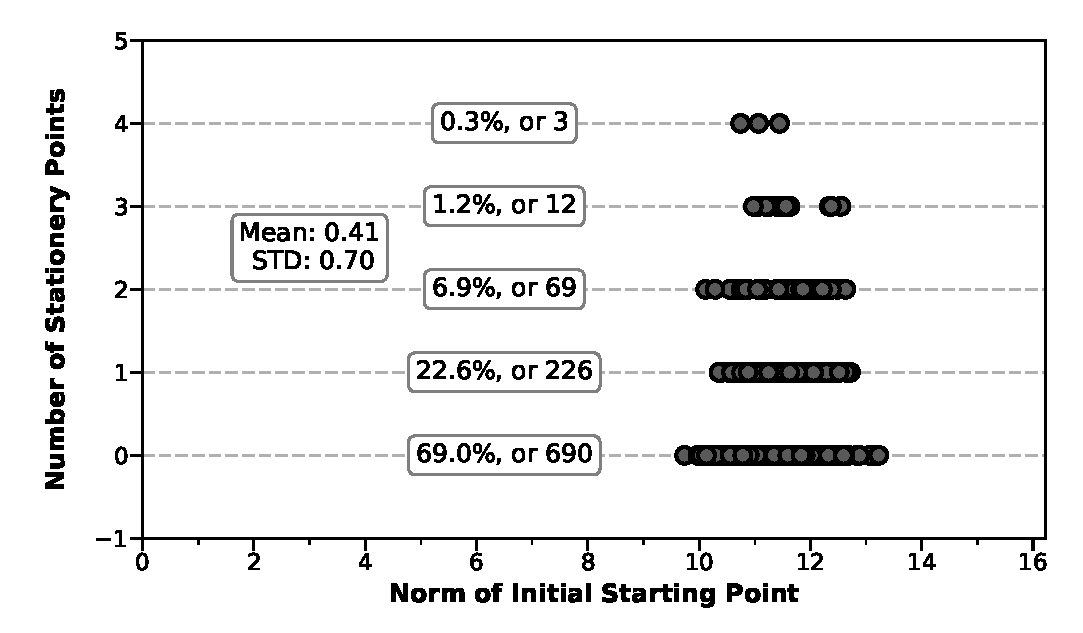
\includegraphics[clip,width=0.7\columnwidth]{./figs/newres2/1000_random.eps}%
  \caption{Stationery Points Distribution. \label{fig:nonconvex}}
\end{figure}

\begin{figure}[tbp]
   \centering
    \subfloat[Convergence vs. $\mu$ \label{fig:ncmu} ]{ 
     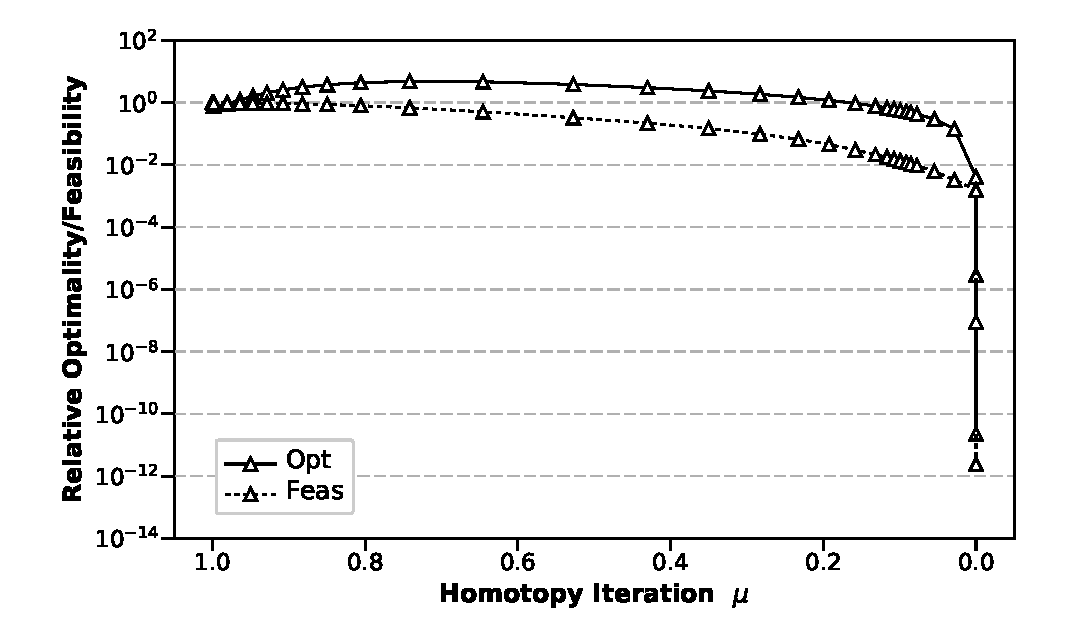
\includegraphics[width=0.7\textwidth]{./figs/newres2/1000_random_mu.eps} } 
     \hspace{1em}
     \subfloat[Convergence vs. CPU time \label{fig:nccpu}]{
     \includegraphics[width=0.7\textwidth]{./figs/newres2/1000_random_cpu.eps} }
    \caption{Typical Convergence Plots in $1000$ Random Cases \label{fig:nc_converg}}
\end{figure}

\begin{remark}
  The parameters $\alpha_0$, $\delta_{\text{targ}}$, $\phi_{\text{targ}}$, and
  $\Delta \mu_{\max}$ all play a role in the ability of Algorithm~\ref{alg:pc}
  to handle nonconvex objectives.  If these parameters are set too agressively,
  then the algorithm may move off the homotopy level-set and converge to a local
  maximizer or saddle, even for the simple problem considered here.
\end{remark}

\section{Scalable quadratic optimization problem}

The next numerical experiement is intended to test the approximate SVD
preconditioner defined in Algorithm~\ref{alg:precond}.  In particular, we are
interested in how this algorithm performs as the number of design variables
increases.  To this end, we consider the following scalable optimization problem
in which we can independently control the size and conditioning of the Hessian
and constraint Jacobian:
\begin{equation*}
  \begin{aligned}
    &\underset{x \in R^n} {\text{min}}  
    & & \frac{1}{2}x^T \mat{Q} x + g^T x \\
    &\text{subject to} & & \mat{A}x \geq b  \\
  \end{aligned}.
\end{equation*}
\padd { The vectors $g\in \mathbb{R}^{n}$ are randomly sampled from a uniform distribution 
in $[ 0,1)$, while $b \in \mathbb{R}^{n}$ from $[0,0.1)$ }

The Hessian $\mat{Q}$ is diagonal with entries
\begin{equation*}
  \mat{Q}_{ii} = \begin{cases}
    \frac{1}{i}, &  i = 1, 2, ...,  \kappa, \\
    \frac{1}{\kappa}, & i = \kappa,  \kappa+1, ... , n, \\
  \end{cases}
\end{equation*}
where $\kappa \leq n$.  This definition produces a Hessian with a condition
number of $\kappa$. \padd{This definition produces a Hessian whose condition number
stays the same as the dimension of the problem increases from $100$ to $500$. }

\padd{
The constraint Jacobian $\mat{A} \in \mathbb{R}^{n\times n}$ is defined as follows. Suppose
$\mat{D} \in \mathbb{R}^{n\times n}$ is a diagonal
matrix of singular values defined similar to $\mat{Q}$:
\begin{equation*}
  \mat{D}_{ii} = \begin{cases}
    \frac{1}{i}, &  i = 1,2,...,\nu, \\
    \frac{1}{\nu}, & i = \nu, \nu+1, ..., n, \\
  \end{cases}
\end{equation*}
where $\nu \leq n$.  Then, $\mat{A}_L $ and $\mat{A}_R$ are matrices of random integers from 
the discrete uniform distribution in the
interval [0,10),  which are applied with $QR$ factorizations,  
\begin{equation*}
\begin{aligned}
\mat{A}_L &= \mat{Q}_L \mat{R}_L \\
\mat{A}_R &= \mat{Q}_R \mat{R}_R \\
\end{aligned}
\end{equation*}
The constraint Jacobian $\mat{A} =\mat{Q}_L  \mat{D} \mat{Q}_R $ 

Consequently, the condition number of $\mat{A}$ is also constant when the dimension 
of the problem increases. 
}

\padd{For this study we chose $\kappa = \nu = 8$, which gives the condition number 
$ \text{cond} (\mat{Q} )= 9$,  $ \text{cond} (\mat{A}) = 81$. The modest condition number of 
$\mat{Q} $ and $\mat{A}$ shifts the focus to treating the ill-condition in the KKT matrix 
$\nabla_{q} F(q)$ at $\mu=0$, whose typical condition number ranges from $1e4$ to $1e9$
depends on the problem.}

The values of $\kappa$ and $\nu$ are randomly chosen to be a fixed positive
value smaller than the number of design variables.  This is to make the
condition number of the matrix fixed, rather than hugely increasing with the
dimension of the problem.

%Although the number of constraints is equal to the number of design variables,
%$n$, the random
\begin{remark}
Although the matrices for this synthetic problem are available explicitly, our
algorithm does not exploit this and remains matrix-free, \ie it only uses
matrix-vector products.
\end{remark}

Figure~\ref{fig:quad_hist} plots the relative optimality and feasibility
histories for the proposed algorithm versus CPU time; the optimality and
feasbility metrics are defined as they were previously for the nonconvex
problem.  The predictor-corrector algorithm is applied both with and without the
approximate SVD preconditioner.  In addition, the plots include the results
obtained using SNOPT~\cite{gill:2002}, a well-validated active-set SQP
optimization library.

Without the preconditioner, the predictor-corrector algorithm is not competitive
and does not converge within X iterations.  This illustrates the need for preconditioning Newton-Krylov
optmization algorithms, even for relatively modest sized problems.  The results
also indicate that the proposed algorithm outperforms SNOPT on this particular
problem.  SNOPT is able to establish feasiblity within the same time as the
predictor-corrector algorithm, but it takes significantly longer to converge the
first-order optimality conditions.

\begin{figure}[tbp]
  \centering
  \subfloat[$n=200$\label{fig:quad_200}]{
   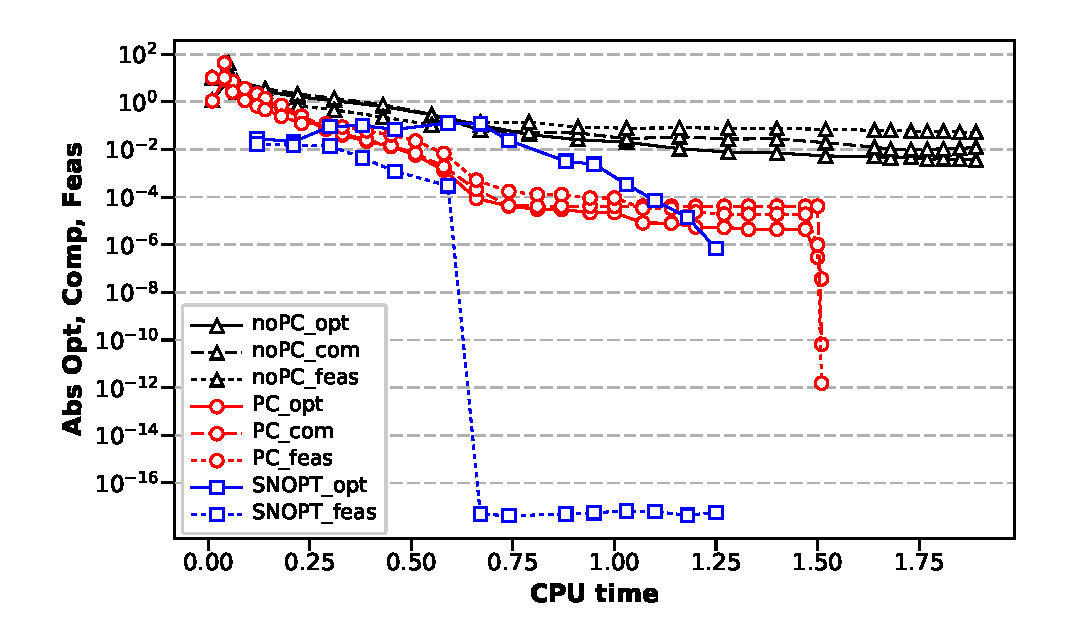
\includegraphics[clip,width=0.7\linewidth]{./figs/newres2/quadratic_200_color.eps} }
   \hspace{1em}
   \subfloat[$n=500$\label{fig:quad_500}]{
   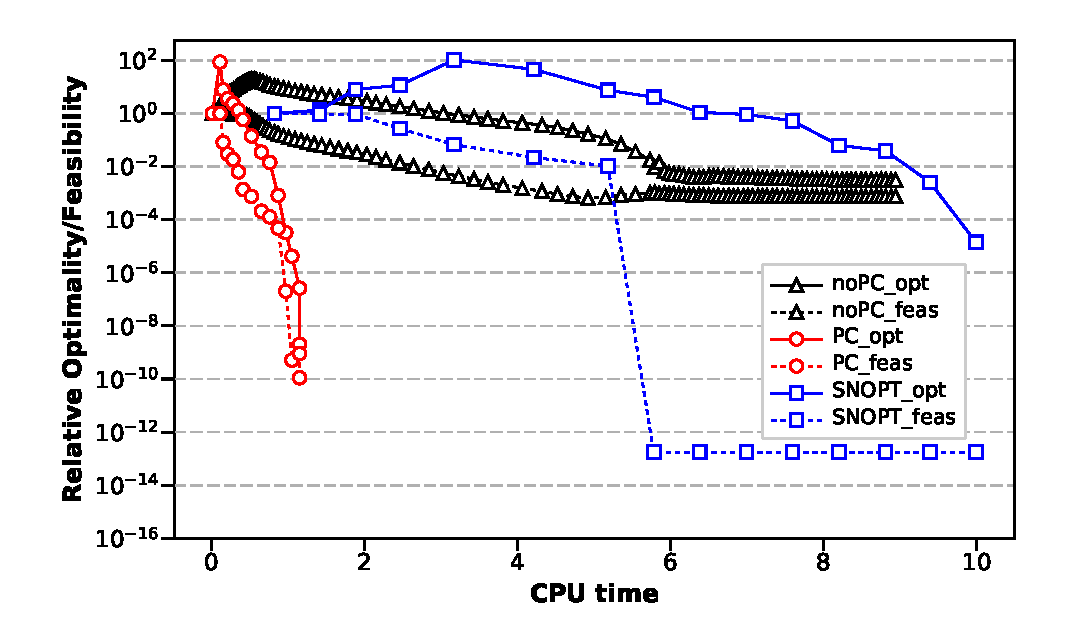
\includegraphics[clip,width=0.7\linewidth]{./figs/newres2/quadratic_500_color.eps} }
   \caption{Convergence histories for the quadratic problem with $n=200$ and
  $n=500$. The results for the proposed algorithm, with and without
  preconditioning, are plotted together with the results from
  SNOPT.\label{fig:quad_hist}}
\end{figure}


To further explore the scalability of the proposed algorithm,
Figure~\ref{fig:quad_scale} plots the total CPU time required by the
preconditioned predictor-corrector algorithm and SNOPT to converge the quadratic
problem as a function of the number of design variables.  For this problem, the
cost of the proposed algorithm grows modestly with $n$ relative to SNOPT.

\begin{figure}[tbp]
  \centering
  \includegraphics[clip,width=0.8\textwidth]{./figs/newres2/quadratic_random_100.eps}%
  \caption{CPU cost versus number of design variables for the quadratic
    optimization problem.\label{fig:quad_scale}}
\end{figure}











%%%%%%%%%%%%%%%%%%%%%%%%%%%%%%%%%%%%%%%%%%%%%%%%%%%%%%%%%%%%%%%%%%% 
%                                                                 %
%                            CHAPTER FIVE                        %
%                                                                 %
%%%%%%%%%%%%%%%%%%%%%%%%%%%%%%%%%%%%%%%%%%%%%%%%%%%%%%%%%%%%%%%%%%% 
 
\chapter{Cuter Test Problems}
\section{Problem Description}\label{sec:cuter1}
The \textbf{CUTEr} Test Problem Set~\cite{cuter_opt, cuter_gould} is a huge collection of test problems to test new optimization codes and develop new algorithms. The problem set ranges from small differentiable unconstrained problem to large scale dense and sparse problems with both equality and inequality constraints, nonlinear systems, and network problems etc.  Some of the test problems exhibit numerical difficulties observable in practice like bad scaling in objective and constraint functions, ill-conditioned problems, multiple local solutions, non-regular solutions where the constraint qualification is not satisfied etc. A number of optimization packages have interfaced with CUTEr~\cite{cuter_interface} like Ipopt, Knitro, Minos, SNOPT etc.  

The problems are written in Standard Input Format (SIF)~\cite{Conn1992}. A decoder works to translate the problems written in SIF to data files in Fortran77, which would provide tools to access the function values, Jacobians, and sometimes Hessians to the optimization packages. It is important for a developing optimization algorithm to test on a good, quality, and suitable subset of problems in CUTEr/CUTEst to validate its accuracy and robustness. 

\subsection{A quick introduction to CUTEr test problems}\label{sec:cuternm}
CUTEr provides access to the objective function and the constraint function, together with the gradients for the test problems. The objective value is a real scalar: 
\begin{equation*}
y = f(x) 
\end{equation*}
where  $x \in \mathbb{R}^n, y \in \mathbb{R}$. $x_i$ is the i-th component of x. 

The constraints include bound constraints on the variable and other types of constraints. The variable $x$ are subject to simple bounds:
\begin{equation*}
\text{bl}_i \leq x_i \leq \text{bu}_i  
\end{equation*}
where $\text{bl}_i$ and $\text{bu}_i$ are the lower and upper bound on $x_i$. When there is no lower or upper bound on $x_i$, then $\text{bl}_i = -1e20$ or $\text{bu}_i = 1e20$. 

Besides bound constraints, all the other constraints are gathered in a single vector-valued function $c(x) \in \mathbb{R}^m$, and constrained in the form:    
\begin{equation*}
\text{cl}_i \leq c_i(x) \leq \text{cu}_i  
\end{equation*}
where either $\text{cl}_i$ or $\text{cu}_i$ is always infinite. This means that the inequality constraint must take just one of the form below for a certain problem:
\begin{equation*}
c_i(x) \geq 0   \quad  \text{or}  \quad  c_i(x) \leq 0
\end{equation*}

For equality constraints $\text{cl}_i$ and $\text{cu}_i$ are both equal to 0. There is also a bool vector $\text{Equatn} \in \mathbb{R}^m$ indicating whether a constraint is an equality constraint or not. 

It is possible to order CUTEr to place equality constraints before inequality constraints, or linear constraints before nonlinear constraints by reordering the components of $c(x)$. Likewise, components of $x$ can be reordered such that nonlinear variables appear before linear ones. 

In addition, CUTEr also outputs the Lagrangian function value, the gradient of the objective function and the Lagrangian, the Jacobian matrix and the Hessian matrix of the constraints. 

\subsection{Kona-CUTEr Interface}
By using a python interface to CUTEr~\cite{cuter_python}, one can access the test problems in Python environment and build the Kona-CUTEr interface. As described in~\cite{dener:scitech2016}, a Kona solver interface essentially asks for matrix-vector products with the system matrix for PDE solvers, and matrix-vector products with constraint Jacobians for equality and inequality constraints separately. As CUTEr test problems do not possess state vectors, and not governed by physics system, the matrix-vector products with the system matrix for PDE solvers are not needed. For the constraint Jacobian products, the explicit Jacobian matrices from CUTEr can be readily used to calculate their products with an arbitrary incoming vector. 

As discussed in chapter \ref{sec:kona_mv}, Kona might not be able to solve CUTEr problems as fast as conventional optimization methods like SNOPT, because the total Jacobian matrix are readily available in CUTEr problems and there is no state variables.  Nonetheless, CUTEr problems are still valuable to validate Kona's accuracy, and capability to overcome other numerical difficulties, and to handle non-convex problems. 

\subsection{Problem Classification}
Each problem in CUTEr is classified following the Hock and Schittkowski scheme~\cite{cuterScheme} by the string: 
\begin{equation*}
X \ X \ X \ r \ - \ X \ X \ - \ n \ - \ m
\end{equation*}

The first character defines the problem objective function type, with the following options: 
\textbf{U}: undefined, \textbf{C}: constant, \textbf{L}: linear, \textbf{Q}: quadratic, \textbf{S}: sum of squares, \textbf{O}: none of the above. 

The second character defines the constraint function type, with the options: 
\textbf{U}: unconstrained, \textbf{X}: fixed variables, \textbf{B}: bounds on the variables, \textbf{N}: adjacency matrix of a linear network, \textbf{L}: linear, \textbf{Q}: quadratic, \textbf{O}: more general constraints. 

The third character shows the smoothness of the problem, with the option of \textbf{R} indicating the problem is regular, and its first and second derivatives exist and continuous everywhere; and \textbf{I}: the problem is irregular. The third character \textbf{r} holds an integer among 0, 1 and 2, indicating the highest derivatives provided analytically.

The first character after the hyphen indicates the origin of the problem, with the option of \textbf{A}: the problem is academic, mainly used by researchers to test algorithms; \textbf{M}: the problem is a modeling exercise, with the solution not used in practical application; \textbf{R}: the solution of the problem has been used in real application.  

The next character shows whether the problem contains internal variables, with the option of \textbf{Y} and \textbf{N}. 

The last two characters \textbf{n} and \textbf{m} indicate the number of variables and constraints (fixed variables and bound constraints excluded) in the problem respectively, with the option of \textbf{V}: an integer chosen by the user, or a constant integer giving the fixed numbers. 

\section{Results}
As the CUTEr test problem set contains a huge collection of problems with assorted features, due to limited time and resources, only a subset of the problems are considered here. Users can select subsets of the problems that belong to a certain category as described in Section~\ref{sec:cuter1} by using Python CUTEr interface. Problems with the following features are selected:
\begin{equation*}
Q \ L \ R \ 2 \ - \ A \ X \ - \ [1,500] \ - \ [1,500]
\end{equation*}
that is, problems with quadratic objective function (convex, non convex, or indefinite), linear constraint function, with second order derivatives and continuous everywhere, from academic area, used by researchers to test algorithms, finally the number of design variables in $[1,500]$ and the number of constraints in $[1,500]$.  Table~\ref{tab:cuter} lists the results on the selected subset of the Cuter problems. The first column 'Name'  are the name of the problems as in \cite{cuter_probs}, where the ascii files are also available that contains information on the problem including problem origin, authors, classifications, SIF problem cards, and sometimes the solutions. The second column 'n, m' are the number of design variable $x$ and constraints as described in~\ref{sec:cuternm}. The third column 'n,  $m_{\text{eq}}$,  $m_{\text{ineq}}$' are the number of $x$, equality constraints and inequality constraints interpreted in Kona's way. The fourth column describes the key word for the origin or origin of the problem. The fifth column lists the major parameters used in the Homotopy RSNK algorithm, the initial step size $\textbf{$\alpha_0$}$, the nominal distance  $\delta_{\text{targ}}$  and nominal angle $\phi^{\circ}_{\text{targ}}$ as defined in Section~\ref{sec:step}, and the rank of the SVD approximation in Lanczos method used in the preconditioner~\ref{eq:svd}. The sixth column is the optimized objective function value using Kona, while the seventh column is that using SNOPT. The last column is the optimized objective function value as shown in the ascii file of~\cite{cuter_probs}. Note that some problems do not provide solutions, thus 'N/A' is used. 

\begin{landscape}
\begin{longtable}{l | l |  l  |  >{\footnotesize}p{3.5cm} | l | c | c | c  }      %\toprule      % |  >{\centering}m{3.5cm}
\caption{Subsets of Cuter Problem Results}\label{tab:cuter} \\
 \hline 
Name   &                 n,   m       &  n,  $m_{\text{eq}}$,  $m_{\text{ineq}}$        &     Origin      &\textbf{$\alpha_0$},  $\delta_{\text{targ}}$, $\phi^{\circ}_{\text{targ}}$,  $\mathbf{{n_{\mat{\Sigma}}}}$      & $ f_{\text{kona}} $   & $ f_{\text{snopt}} $ &$ f^*$    \\ \hline
AUG2D    &           24,  9         &  24,   9,  18       &    2-D Laplace   & 0.05,1,5,30   &  0.124999           &     0.1250    &      N/A                \\ \hline
AUG2D    &          220, 100   & 220, 100, 200  &                      &   0.05,1,5,30         &   110.7987          &    110.7991      &    N/A           \\ \hline
AUG2DC  &       24, 9      &   24, 9, 18       &       &     0.05,1,5,30        &    2.973213        & 2.973214    &   N/A     \\ \hline
AUG2DC  &      220, 100   &  220, 100, 200   &     &   0.05,1,5,30    & 184.2388    &   184.2394     &    N/A      \\ \hline
AUG3D  &      156, 27    & 156, 27, 54   & 3-D Laplace  &  0.05,1,5,30   & 0.08333   &   0.083333   &  N/A         \\ \hline
AUG3DC  &  156, 27  &  156, 27, 54   &    & 0.05,1,5,30 &   35.84226   &   35.84276      & N/A      \\ \hline
AVGASA  &       8, 10   &   8, 0, 26   &            LP problem     &   0.05,1,5,30       &           -4.63092    &    -4.79278   &   N/A     \\ \hline
AVGASB  &    8, 10  &   8, 0, 26   &   LP problem      & 0.05,1,5,30   &   -4.482206   &   -4.666351     &   N/A    \\ \hline
ALLINQP  & 10, 5   &  10, 1, 21   & banded QP  &  0.05,10,20,30 & 0.346667  & -0.183256     &  N/A \\  \hline     %\midrule
BLOCKQP2   & 25, 11   & 25,  10, 71   &    non-convex  & 0.05,1,5,5  & -6.201652   & -2.507e+14    &  -6.2017   \\ \hline
BLOCKQP3   & 25, 11   & 25,  10, 71  &  	  & 0.05,1,5,2 & 2.330508     &  2.330508   &            -2.4987e-1   \\ \hline
BLOCKQP4  & 25, 11    & 25, 10, 71  &    & 0.05,1,5,5     & -2.928928   & -5.73e+14   &    -2.499e-1   \\ \hline
BDRY2   & 25, 18   & 25, 18, 86   &  AMPL  & 0.05,1,5,3  & 0.544932  & 0.548110  & N/A    \\ \hline   
BIGGSC4  & 4, 7   & 4, 0, 21   & & 0.05,1,5,2  & -24.4999   &  -24.375  &    -24.5 \\ \hline 
CVXQP1  & 10, 5 & 10, 5, 30  & convex   & 0.05,1,5,2 & 181.0401 & 165.8738  & N/A   \\ \hline
DEGENQP & 10, 1005 & 10,5,2030  & degenerate convex  & 0.05,1,5,10  & 8.80e-06 & -5.55e-17  & N/A \\ \hline
DTOC3   & 29, 18  & 29,18,40 & discrete time control & 0.05,1,5,10  &  224.5904 & 8.20189  & 224.5904 \\ \hline 
GENHS28 & 10, 8  & 10, 8, 16  & Hock and Schittkowski &   0.05,1,5,2   & 0.927173  & 0.927174  & 0.0   \\ \hline
GMNCASE1 &  175, 300   & 175, 0, 300  &   optimized control   & 0.5, 5, 5, 100   &   0.267087  & 0.266973             &    0.266733   \\ \hline
GMNCASE4 & 175, 350 & 175, 0, 350  &  optimized control &  0.5, 5, 5, 100      & 5.6273e3 &  5.9469e3 &    5.9468e3 \\ \hline 
HS268   & 5,5  & 5, 0, 5  &  Schittkowski   &  0.05,50,5,3    & 2.09e-4   & -3.6e-12      &    N/A    \\ \hline 
HS21    &  2,1 & 2,0,5   & Hock and  Schittkowski  &  0.5,5,10,1   & -99.3434  & -99.9900  & -99.96    \\ \hline 
HS35   &  3,1  & 3,0,4  &             &  0.05,1,5,1    & 0.111111  & 0.111111   &   0.111111   \\ \hline 
HS35I   &  3,1  & 3,0,7  &             &   0.05,1,5,1      & 0.111111  & 0.111111   &   0.111111   \\ \hline 
HS44   & 4,6   & 4,0,10   &  	 & 0.05,1,20,3      &  -13.000 & -4.01e+14 & -13.0    \\ \hline
HS44NEW & 4,6  & 4,0,10  &     &   0.05,1,20,3    & -13     & -3.20e+14   & -13.0    \\ \hline
HS51    &  5,3   & 5,3,6    &  & 0.05,1,20,3      & 4.46e-19   & 5.86E-14     & 0.0    \\ \hline
HS52    &  5,3  & 5,3,6   & & 0.05,1,20,3      & 5.326634   & 5.326647   & 5.326643   \\ \hline
HS53    &  5,3  & 5,3,16    &   &  0.05,1,5,3  & 4.093023   & 4.093023   & 4.093023  \\ \hline
HS118  & 15,17  & 15,0,59  & & 0.05,50,5,3   & 664.8205  & -1748.638  & 664.8204    \\ \hline
HS268  & 5,5  & 5,0,5  & & 0.05,50,5,3     & 3.839e-4 & -3E-12  & N/A   \\ \hline
HATFLDH  & 4, 7 &  4, 0, 21  & & 0.05,1,5,2  &  -24.5002  & -24.375 & 24.5   \\ \hline
LOTSCHD  & 12,7  &  12, 7, 26 & eco. lot scheduling &  0.05,1,5,4   & 44.2890 & 165.6553  & N/A  \\ \hline
MOSARQP1 & 36, 10 & 36, 0, 46 &convex quadratic & 0.05,1,5,4     &  -24.14365 & -52.04917 & -24.13768 \\ \hline
MOSARQP2 &36, 10 & 36, 0, 46 &     & 0.05,1,5,4   & -35.69815  & -55.16234  & -35.6981 \\ \hline
POWELL20 & 10,10  & 10,0,10 & degenerate convex & 0.05,1,5,2    & 57.8125 & 57.8125  & N/A  \\\hline
RDW2D52F & 18,1  & 18,1,36 & optimal control &  0.05,10,20,5 &  0.053016 & 0.020779 & N/A \\\hline
STCQP1  & 17, 8  &  17, 8, 50 & convex   &    0.05,1,5,5  & 494.4054  & 494.5208  & 4.95E+02 \\\hline
SOSQP1 &  20, 11 & 20, 11, 62 & non-convex & 0.05,1,5,2    & 5.9e-07 & -4E-16   & 0.0 \\\hline
SOSQP2 & 20,11  &  20, 11, 62 &    & 0.05,1,5,5	& -3.99779  & -4.04565  & -3.99781    \\\hline
S268   &   5,5   & 5,0,5  &   & 0.05,10,20,10  &   2.274e-3  &  -3.64E-12  & N/A  \\\hline
YAO   &  22,20  & 22, 0, 25 &   &  0.05,1,5,10 & 2.398829  & 3.715e-3 & 2.39883  \\\hline
ZECEVIC2 & 2,2 & 2,0,6  & &  0.05,1,5,2 & -4.1249  & -4.125  & N/A  \\\hline
\end{longtable}   % \midrule
\end{landscape}


As can be seen, for most problems, the proposed Homotopy RSNK method and the preconditioner can deliver accurate solutions.  However, even with a small number of numerical tests, several valuable insights could be drawn: 
\begin{enumerate}
\item While the current Homotopy RSNK optimization algorithm works as a general optimization method, irrelevant of the problem types and feature, it struggles on problems with any hint of ill-conditioning, such as degenerate problems where the constraint qualifications are not satisfied, badly scaled objective and constraint functions. 
\item As CUTEr test problems do not involve the state variables and thus adjoint variables, the Homotopy RSNK's core strength of using second-order adjoints to approximate Hessian vector products is not applicable. In contrast, SNOPT can readily make good use of the explicit Jacobians 
provided by the pyCUTEr tool, while Kona is only using the explicit matrices to calculate the products in order to form the Krylov subspace. Consequently, SNOPT is faster than Kona when solving the CUTEr problems on average.   
\item The proposed matrix-free preconditioner is not general and is specifically designed for PDE-constrained optimization problems as introduced at the beginning of this thesis.  For bound-only constraints, it does not work that well. Because the constraint Jacobians are Identity matrix, the Krylov subspace built from it is only 1-rank, making the Lanczos method's SVD approximation very insufficient.  
\item If the product of the constraint Jacobian with a vector of ones is always zero, then it will make the preconditioner crash. Because the Krylov subspace would be linearly dependent, making the Lanczos methods fail. Problems whose constraint Jacobian has the non-zero entries of e.g. $[-1, -3, 3, 1]$ on each row belong to this category, like the LISWET problems 
\item For non-convex problems, sometimes the proposed Homotopy RSNK can work, and sometimes not. So more effort is needed to increase the robustness of the algorithm. 
\end{enumerate} 

 
 

%%%%%%%%%%%%%%%%%%%%%%%%%%%%%%%%%%%%%%%%%%%%%%%%%%%%%%%%%%%%%%%%%%% 
%                                                                 %
%                           BIBLIOGRAPHY                          %
%                                                                 %
%%%%%%%%%%%%%%%%%%%%%%%%%%%%%%%%%%%%%%%%%%%%%%%%%%%%%%%%%%%%%%%%%%% 

\specialhead{REFERENCES}
%\bibliographystyle{unsrt} % specify bibliography style
\bibliographystyle{IEEEtran_rpi}
\begin{singlespace}
\bibliography{mengp2}  % Prints the bibliography here, using "myrefs.bib"
\end{singlespace}

%This method produces a numbered bibliography where the numbers
%correspond to the \cite commands in the text. See the LaTeX manual.
%
% epstopdf

%\specialhead{REFERENCES}
%\begin{singlespace}
%\begin{thebibliography}{99}
%\bibitem{thisbook} This is the first item in the Bibliography.
%\bibitem{anotherbook} The second item in the Bibliography.
%\bibitem{yetanotherbook} Another item in the Bibliography.
%\end{thebibliography}
%\end{singlespace}

% Note that, if you wish, you can use BibTeX to create your bibliography
% from a database. See section 5.6.2 of Memo RPI.110 for information. 
%%% Local Variables: 
%%% mode: latex
%%% TeX-master: t
%%% End: 

%Just remember that to create the bibliography, 
%you must run LATEX, then BibTEX, then run LATEX twice more.
   
%%%%%%%%%%%%%%%%%%%%%%%%%%%%%%%%%%%%%%%%%%%%%%%%%%%%%%%%%%%%%%%%%%%
%                                                                 %
%                            APPENDICES                           %
%                                                                 %
%%%%%%%%%%%%%%%%%%%%%%%%%%%%%%%%%%%%%%%%%%%%%%%%%%%%%%%%%%%%%%%%%%%
 
\appendix    % This command is used only once!
%\addcontentsline{toc}{chapter}{APPENDICES}             %toc entry  or:
\addtocontents{toc}{\parindent0pt\vskip12pt APPENDICES} %toc entry, no page #

\chapter{THIS IS AN APPENDIX}

\begin{landscape}     % ADD CUTER PROBLEM SETTNGS!  refer to this table for all problems involved!!
\begin{longtable}{ l c c c c c c c }
%  \begin{center}
    \caption{Parameters used in the test problems \label{tab:param}} \\
    \textbf{Parameters} & $\textbf{Default}$     & $\textbf{Range}$ &  $\textbf{Sphere}$    &   $\textbf{Non-convex}$ 
    & $ \textbf{Quadratic} $   & \textbf{Structural}    &  \textbf{ASO} \\ \hline
    %\rule{0ex}{3ex}%
    \multicolumn{8}{ l }{Predictor-Corrector Algorithm} \\   %  $\delta_{\text{targ}}$ and $\phi_{\text{targ}}$. 
    \hline    
    $K_{\max}$             	&  100     & $\geq$100   & 500      & 100 	 &  100       &    100  & 100    \\ 
     $J_{\max}$  		&   2         & $\geq$2         & 2    & 2          & 2           &      2     & 2   \\
    $\epsilon_F$ 	           		&  1e-6     & [1e-8, 1e-3]    & 1e-7   & 1e-7 	 & 1e-7       &    1e-4   & 1e-3  \\ 
       $\tau$    		&   0.1      & [0.1,0.5]	    & 0.1    & 0.1          & 0.1	 &     0.1   & 0.1  \\
    $\epsilon_H$    		&   0.1      & [0.1,0.5]	    & 0.1       & 0.1          & 0.1	 &     0.1   & 0.1    \\
   % $\epsilon_{\mu} $   & 1e-9     & [1e-10, 1e-6]   &   &   1e-9  & 1e-9  & 1e-6  &  \\   
    \textbf{$\alpha_0$}             &  0.05     & $\geq$0.01    & 0.05      & 0.05	 & [40,60,80,100,120]  &  0.05  & 0.05 \\
    $\delta_{\text{targ}}$      &  1.0	& [1.0,10]       & 1	    & 10		 & 10    &   1.0   & 10	  \\
    $\phi^{\circ}_{\text{targ}}$   & 10.0	& [5.0,50] 	     & 10     & 10		 & 20    &   10    & 20    \\
    $\zeta_{\max}$ 		        &  50		& [10,50]	& 50       & 50		 & 50    	 &   50   & 50  \\
    $\zeta_{\min}$ 		        &  0.5	& 0.5		& 0.001       & 0.001	 & 0.001    &   0.5  & 0.001 \\
    $\Delta \mu_{\max}$		        &  -5e-4	& [-5e-4, -5e-1] & -5e-4 & -5e-4	 & -5e-4     &  -5e-4 & -5e-4 \\  
    $\Delta \mu_{\min}$		        &  -0.9	& -0.9 	& -0.9	       & -0.9		 & -0.9       &  -0.9  & -0.9	  \\
    $s_0$                           & $\mathbf{e}$     &   $>$ 0  & $g(x_0)$  &    5$\mathbf{e}$    &  10$\mathbf{e}$   &  $g(x_0)$  & $g(x_0)$  \\ 
    $\tau_s$                      & 1e-6    & 1e-6    &  1e-6 &  1e-6   &  1e-6    & 1e-6  &  1e-6 \\
    \hline
    \multicolumn{8}{ l }{Preconditioner} \\ 
    \hline    
    $\mathbf{{n_{\mat{\Sigma}}}}$    & 5	       & $\geq$2	  & -    &  -	         &  2       &  [20,80,320]   & 20 \\
    $\beta$				& 1.0	       & $>$0        & -      & -    &  -      &  0.1 & -  \\
    $N_{\text{bfgs}}$		& 10	       & [1, 20]		& - 	&  -   	 &  10	& -     &  20    \\
    $\mu_e$			& -1	       & [0, 1] 	& -	& -	         &  -	        & 1e-3  & 1e-3\\
    $\Sigma_e$			& 1 	       & [0, 1]      & -           & -		& -		& 1e-3 & - \\
    \hline
    \multicolumn{8}{ l }{Krylov Iterative Solver} \\ 
    \hline       
    $n_k$		& 20        & [10,30]              & 20	 & 20	 &  20       &  20   & 20  \\
    $\epsilon_{\text{krylov}}$		& 1e-2     & [0, 0.1]    &1e-2       	&1e-2	 &  1e-2    &  1e-4  &1e-2\\
    \hline
%  \end{center}
\end{longtable}    
\end{landscape}



\section{Brief overview of the CUTEr test problems}\label{sec:cuternm}
For each test problem, CUTEr provides access to the objective function and the constraint functions, as well as their derivatives.
% The objective value is a real scalar: 
%\begin{equation*}
%y = f(x) 
%\end{equation*}
%where  $x \in \mathbb{R}^n, y \in \mathbb{R}$. $x_i$ is the i-th component of x. 

The constraints include bound constraints on the variable and other types of constraints. The variable $x$ are subject to simple bounds:
\begin{equation*}
\text{bl}_i \leq x_i \leq \text{bu}_i  
\end{equation*}
where $\text{bl}_i$ and $\text{bu}_i$ are the lower and upper bound on $x_i$. When there is no lower or upper bound on $x_i$, then $\text{bl}_i = -1e20$ or $\text{bu}_i = 1e20$. 

With the exception of the bound constraints, all remaining 
constraints are gathered in a single vector-valued function $c(x) \in \mathbb{R}^m$, which is then bounded as follows:   
\begin{equation*}
\text{cl}_i \leq c_i(x) \leq \text{cu}_i  
\end{equation*}
where one of $\text{cl}_i$ or $\text{cu}_i$ is always around $10^{20}$. This means that the inequality constraint must take just one of 
the following two forms on a given problem:
\begin{equation*}
c_i(x) \geq 0   \quad  \text{or}  \quad  c_i(x) \leq 0.
\end{equation*}
For equality constraints $\text{cl}_i$ and $\text{cu}_i$ are both equal to 0. There is also a bool vector, $\text{Equatn} \in \mathbb{R}^m$, indicating whether a constraint is an equality constraint or not. 

It is possible to instruct CUTEr to order equality constraints before inequality constraints, or linear constraints before nonlinear constraints, by reordering the components of $c(x)$. Likewise, components of $x$ can be reordered such that nonlinear variables appear before linear ones. 

In addition, CUTEr can also output 
the Lagrangian function value, the gradient of the objective function and the Lagrangian, the Jacobian matrix and the Hessian matrix of the constraints. 

\section{Kona-CUTEr Interface}\label{sec:konacut}
By using a Python interface to CUTEr~\cite{cuter_python}, one can access the test problems in Python environment and build the Kona-CUTEr interface. As described in~\cite{dener:scitech2016}, a Kona solver interface essentially asks for matrix-vector products with the PDE-Jacobian (if any),  
 and matrix-vector and vector-matrix products with the Jacobians of the equality and inequality constraints. 
The explicit Jacobian matrices from CUTEr can be readily used to calculate their product with an arbitrary incoming vector for Kona.  CUTEr problems are still valuable to verify Kona's accuracy, as well as its capability to overcome other numerical difficulties, including non-convex problems. 

%As discussed in chapter \ref{sec:kona_mv}, Kona might not be able to solve CUTEr problems as fast as conventional optimization methods like SNOPT, because the Jacobians are explicitly available in CUTEr problems.  


\section{Problem Classification}\label{sec:cuter_clas}
Each problem in CUTEr is classified following the Hock and Schittkowski scheme~\cite{cuterScheme} by the string: 
\begin{equation*}
X \ X \ X \ r \ - \ X \ X \ - \ n \ - \ m
\end{equation*}

The first character defines the problem objective function type, with the following options: 
\begin{itemize}  \itemsep -8pt 
\item \textbf{U}: undefined,
\item  \textbf{C}: constant, 
\item \textbf{L}: linear, 
\item \textbf{Q}: quadratic, 
\item  \textbf{S}: sum of squares, 
\item  \textbf{O}: none of the above. 
\end{itemize}

The second character defines the constraint function type, with the options: 
\begin{itemize}  \itemsep -8pt 
\item  \textbf{U}: unconstrained,
\item  \textbf{X}: fixed variables, 
\item  \textbf{B}: bounds on the variables,
\item  \textbf{N}: adjacency matrix of a linear network,
\item  \textbf{L}: linear, 
\item  \textbf{Q}: quadratic,
\item  \textbf{O}: more general constraints. 
\end{itemize}

The third character shows the smoothness of the problem, with the option of:
\begin{itemize}  \itemsep -8pt 
\item  \textbf{R} : the problem is regular, and its first and second derivatives exist and continuous everywhere,
\item  \textbf{I}: the problem is irregular.
\end{itemize}

The third character \textbf{r} holds an integer among 0, 1 and 2, indicating the highest derivatives provided analytically.

The first character after the hyphen indicates the origin of the problem, with the option of:
\begin{itemize}  \itemsep -8pt 
\item  \textbf{A}: the problem is academic, mainly used by researchers to test algorithms; 
\item  \textbf{M}: the problem is a modeling exercise, with the solution not used in practical application; 
\item  \textbf{R}: the solution of the problem has been used in a real application.  
\end{itemize}

The next character has an option of: 
\begin{itemize}  \itemsep -8pt 
\item \textbf{Y}: the problem contains internal variables, 
\item \textbf{N}: the problem does not contain internal variables. 
\end{itemize}

The last two characters have the following options:
\begin{itemize}  \itemsep -8pt 
\item \textbf{n} - \textbf{m}: the number of variables and constraints (fixed variables and bound constraints excluded), 
\item \textbf{V} - \textbf{V}: an integer chosen by the user among the given list of fixed numbers.
\end{itemize}


\section{A Section Heading}

This is how equations are numbered in an appendix:
\begin{equation}
x^2 + y^2 = z^2
\end{equation} 
This is a sentence to take up space and look like text.

\chapter{THIS IS ANOTHER APPENDIX} 
This is a sentence to take up space and look like text.
 
%\include{99-appendix}
\end{document}

